\documentclass[10pt,letterpaper]{article}

% --- Paquetes Esenciales ---
\usepackage[utf8]{inputenc}
\usepackage[spanish,es-tabla]{babel}
\usepackage[margin=1.7cm,top=1.8cm,bottom=1.8cm]{geometry}
\usepackage{amsmath,amssymb,amsfonts}
\usepackage{booktabs}
\usepackage{graphicx}
\usepackage{float}
\usepackage{subcaption}
\usepackage{xcolor}
\usepackage{hyperref}
\usepackage{enumitem}
\usepackage{titlesec}
\usepackage{microtype}
\usepackage{fancyhdr}
\usepackage{cite}

% --- Colores Institucionales y Enlaces ---
\definecolor{usmblue}{RGB}{0,51,102}
\definecolor{darkgray}{RGB}{50,50,50}

\hypersetup{
    colorlinks=true,
    linkcolor=usmblue,
    citecolor=usmblue,
    urlcolor=usmblue
}

% --- Encabezados y Pies de Página ---
\pagestyle{fancy}
\fancyhf{}
\fancyhead[L]{\small\color{darkgray}\textit{ILN250 -- Investigación de Operaciones (2s26)}}
\fancyhead[R]{\small\color{darkgray}\textit{Tarea Computacional 1: Unit Commitment}}
\fancyfoot[C]{\thepage}
\renewcommand{\headrulewidth}{0.4pt}
\renewcommand{\footrulewidth}{0.4pt}

% --- Configuración de Títulos ---
\titleformat{\section}{\large\bfseries\color{usmblue}}{\thesection.}{0.4em}{}
\titleformat{\subsection}{\normalsize\bfseries\color{usmblue}}{\thesubsection.}{0.3em}{}
\titleformat{\subsubsection}{\small\bfseries\color{darkgray}}{\thesubsubsection.}{0.25em}{}
\titlespacing*{\section}{0pt}{1.0ex plus 0.3ex minus 0.2ex}{0.4ex plus 0.2ex}
\titlespacing*{\subsection}{0pt}{0.8ex plus 0.3ex minus 0.2ex}{0.3ex plus 0.1ex}
\titlespacing*{\subsubsection}{0pt}{0.6ex plus 0.2ex minus 0.1ex}{0.2ex plus 0.1ex}

\setlist[itemize]{noitemsep, topsep=1.5pt, parsep=0.5pt, leftmargin=1.5em}
\setlist[enumerate]{noitemsep, topsep=1.5pt, parsep=0.5pt, leftmargin=1.5em}

\begin{document}

% =========================================================================
% PORTADA (No cuenta dentro de las 10 páginas)
% =========================================================================
\begin{titlepage}
    \centering
    \vspace*{0.8cm}
    {\large Investigación de Operaciones (ILN250)\par}
    \vspace{2.0cm}
    
    \rule{\linewidth}{1.2pt} \\[0.4cm]
    {\huge\bfseries\color{usmblue} Tarea Computacional 1: \\[0.25cm]}
    \rule{\linewidth}{1.2pt} \\[2.0cm]
    
    \begin{minipage}[t]{0.48\textwidth}
        \textbf{Profesor:}\\
        Rafael Favereau U.\\
    \end{minipage}
    \hfill
    \begin{minipage}[t]{0.48\textwidth}
        \raggedleft
        \textbf{Integrantes:}\\
        Cristobal Cortés\\
        Luciano Ferroni\\[0.2cm]
        \textbf{Semilla de Grupo:}\\
        $392 + 142 =$ \textbf{534}\\[0.2cm]
    \end{minipage}
    
    \vfill
    {\large Valparaíso, Chile \\ Septiembre de 2026 \par}
\end{titlepage}

% =========================================================================
% FRONT MATTER (Páginas preliminares en números romanos)
% =========================================================================
\pagenumbering{roman}
\setcounter{page}{1}

\section*{Resumen Ejecutivo}
\addcontentsline{toc}{section}{Resumen Ejecutivo}

El presente informe aborda el modelamiento, resolución computacional y análisis del problema de \textit{Unit Commitment} (UC) y Despacho para un complejo industrial eléctricamente aislado durante un horizonte temporal semanal de 168 horas.

La micro-red cuenta con un parque de generación térmica heterogéneo $|G| = 5$ (dos unidades a gas de base, dos grupos diésel de modulación intermedia y una turbina peaker de punta) junto a un enlace limitado con el mercado eléctrico externo ($\bar{G}_{red} = 80$ MW) sujeto a precios horarios volátiles $\lambda_t$. El problema se formula como un Programa Lineal Entero Mixto \textit{MILP}, integrando costos de generación, arranque (\textit{start}), costos fijos de operación (\textit{no-load}), dinámicas de rampa horaria con excepciones al arranque/parada, y reserva operativa del 10\% de la demanda. La implementación se llevó a cabo en Python con \textbf{Pyomo}, resolviéndose mediante el solver \textbf{HiGHS} (\texttt{appsi\_highs}), para entontrar la solución óptima global.

Los principales hallazgos del estudio comprenden:
\begin{enumerate}
    \item \textbf{Situación Inicial (Caso Base):} El costo total de operación semanal asciende a \textbf{\$1.776.019.094,00 CLP}. La estructura de costos se desglosa en: 93,73\% por costos variables de generación (\$1.664.741.000 CLP), 5,63\% por costos de no-load (\$100.060.000 CLP), 0,44\% por partidas térmicas (\$7.800.000 CLP) y 0,19\% por importación de red (\$3.418.094 CLP). El orden de mérito económico demuestra que las unidades a gas (\texttt{Gas\_Base\_1} y \texttt{Gas\_Base\_2}) absorben la base con factores de planta del 95,9\% y 72,7\%, respectivamente. La unidad \texttt{Diesel\_Med\_1} modula la carga diurna laboral (FP 23,6\%, 5 arranques), mientras que \texttt{Diesel\_Med\_2} y \texttt{Peaker} se reservan exclusivamente para los picos extremos de demanda ($FP \le 0,5\%$). La importación de red es muy reducida (18,0 MWh en 6 horas), confirmando que la red se emplea únicamente como respaldo de confiabilidad ante restricciones de rampa y reserva en horas punta.
    \item \textbf{Variación 2.a (Sistema con Batería):} La incorporación de un sistema de almacenamiento de energía genera un ahorro económico neto de \textbf{\$43.973.254,66 CLP semanal (2,48\% de reducción)}, alcanzando un costo de \$1.732.045.839,34 CLP. La batería es capaz de almacenar 1.225,5 MWh nocturnos e inyectar 1.106,0 MWh en horas punta. La batería **elimina en un 100\% las importaciones de la red externa** (0 MWh) y suprime totalmente los arranques de las unidades más costosas (\texttt{Diesel\_Med\_2} y \texttt{Peaker}).
    \item \textbf{Variación 2.b (Respuesta de Demanda):} El análisis paramétrico de sensibilidad respecto al costo de interrupción $c^{shed}$ reveló un umbral económico crítico exacto de \textbf{\$200.000 CLP/MWh}. A partir de este valor, el recorte se anula por completo ($r_{total} = 0$ MWh). Este umbral coincide con el costo marginal máximo de importación de la red externa durante el peak vespertino, ratificando analíticamente los principios de formación de precios y despacho marginal.
    \item \textbf{Variación 2.c (Umbral de Emisiones con Big-M):} Frente a una penalización fija diaria $F$ por superar 1.500 $\text{tCO}_2$, se identificó que en el caso base los días sábado y domingo ya cumplen naturalmente con el umbral ($1.483,8$ y $1.487,2\text{ tCO}_2$). En días laborales, abatir las emisiones exige importar al máximo técnico de la red (80 MW las 24 horas), lo que impone un sobrecosto superior a \$108 millones CLP diarios por día hábil. En consecuencia, el sistema reduce a 2 días infractores recién a $F = \$100.000.000$ CLP/día y alcanza 0 días sobre el umbral a $F \ge \$120.000.000$ CLP/día, disparando el costo operativo semanal en más de \$500 millones CLP, demostrando la distorsión económica que introducen las sanciones de tipo umbral discontinuo frente a tributos continuos al carbono.
\end{enumerate}

\newpage
\tableofcontents
\newpage

\pagenumbering{arabic}
\setcounter{page}{1}

\section{Introducción General}
\label{sec:introduccion}

El problema abordado en esta investigación corresponde a la planificación operativa semanal ($T = 168$ horas) de un complejo industrial aislado provisto de un parque térmico heterogéneo de cinco unidades ($|G| = 5$) y un enlace de capacidad acotada ($\bar{G}_{red} = 80$ MW) con el mercado eléctrico externo. La optimización del despacho requiere resolver simultáneamente dos decisiones interdependientes:
\begin{enumerate}
    \item \textbf{Unit Commitment (Decisión Binaria):} Determinar qué unidades generadoras deben encenderse, mantenerse en línea o apagarse en cada intervalo horario, incurriendo en costos fijos de operación (\textit{no-load}) y costos de arranque (\textit{startup}).
    \item \textbf{Despacho Económico (Decisión Continua):} Asignar la potencia generada por cada unidad en servicio y la cantidad de energía importada desde la red externa a precio horario $\lambda_t$, satisfaciendo el balance instantáneo de energía, límites de capacidad técnica, restricciones de velocidad de cambio de carga (rampas de subida y bajada) y márgenes de reserva operativa ante contingencias.
\end{enumerate}

El objetivo central del presente estudio es formular el modelo matemático óptimo para el caso base, resolverlo computacionalmente mediante herramientas de programación matemática en Python (Pyomo), e investigar cuantitativamente el impacto de tres variaciones tecnológicas y regulatorias: (i) almacenamiento de energía, (ii) respuesta de demanda con carga interrumpible, y (iii) una política ambiental con penalización fija diariapor sobrepasar un umbral de emisiones de $\text{CO}_2$.

\section{Supuestos}
\label{sec:supuestos}

Para garantizar un modelamiento matemáticamente riguroso, consistente y computacionalmente tratable, se establecen los siguientes supuestos operativos:

\begin{enumerate}
    \item \textbf{Discretización Temporal y Régimen Cuasi-Estacionario:} El horizonte semanal se discretiza en 168 bloques horarios independientes de $\Delta t = 1$ hora. La potencia promedio en MW durante una hora equivale numéricamente a la energía entregada en MWh. Las variables representan el estado promedio en cada bloque horario.
    \item \textbf{Estructura de Costos Térmicos:} Los costos de operación se separan en tres componentes:
    \begin{itemize}
        \item \textit{Costo Variable ($c_g^{var}$):} Costo proporcional a la energía eléctrica generada [CLP/MWh].
        \item \textit{Costo de No-Load ($c_g^{nl}$):} Costo fijo horario [CLP/h] en el que incurre cada generador por mantenerse encendido, independiente de su nivel de despacho.
        \item \textit{Costo de Arranque ($c_g^{start}$):} Costo monetario fijo por encender un generador. El costo de detención se asume nulo ($c_g^{stop} = 0$).
    \end{itemize}
    \item \textbf{Dinámica de Rampas y Ajuste al Arranque/Parada:} Se restringen las variaciones de potencia a un máximo de $R_g$ MW/h entre horas consecutivas. Cuando la unidad arranca, puede alcanzar hasta $\max(P_g^{min}, R_g)$ MW para no restringir artificialmente a unidades con $R_g > P_g^{min}$ (ej. diésel y peaker) ni provocar infactibilidad en unidades donde $P_g^{min} > R_g$ (como las turbinas a gas). Análogamente, antes de apagarse, la unidad desciende a lo más hasta dicho umbral.
    \item \textbf{Condiciones Iniciales del Sistema ($t=0$):} Se establece que las dos unidades de base (\texttt{Gas\_Base\_1} y \texttt{Gas\_Base\_2}) inician encendidas a su mínimo técnico ($u_g^0 = 1$, $p_g^0 = P_g^{min}$), mientras que las unidades intermedias y peaker inician apagadas ($u_g^0 = 0$, $p_g^0 = 0$). Estas condiciones gobiernan los arranques y rampas de la hora $t=1$.
    \item \textbf{Reserva Operativa y Seguridad de Suministro:} Por seguridad, se exige en todo momento una reserva mínima $Res_t = \lfloor 0.10 \cdot d_t \rceil$, provista conjuntamente por la capacidad disponible no despachada de máquinas encendidas y la holgura del enlace de red ($\bar{G}_{red} - g_t^{red}$).
    \item \textbf{Operación de Almacenamiento (BESS):} Se asume eficiencia de carga $\eta^{ch} = 0.95$ y descarga $\eta^{dis} = 0.95$. Dado que los costos marginales de generación y precios de red son estrictamente positivos, la optimización económica descarta de forma natural la carga y descarga simultánea sin requerir variables binarias adicionales.
    \item \textbf{Perímetro de Emisiones:} El umbral de $1.500 \text{ tCO}_2$/día aplica exclusivamente a las emisiones directas del complejo.
\end{enumerate}

\section{Situación Inicial}
\label{sec:situacion_inicial}

\subsection{Pregunta 1.a: Generación de Parámetros y Perfiles de Instancia}
\label{subsec:1a}

La demanda horaria $d_t$ y el precio de red $\lambda_t$ se obtuvieron mediante el generador estocástico parametrizado con la semilla 534 conforme a las expresiones:
\begin{equation}
    d_t = \left\lfloor P^{peak} \cdot \gamma_{dia(t)} \cdot s_{h(t)} \cdot (1 + \varepsilon_t) \right\rceil, \quad 
    \lambda_t = \left\lfloor (100.000 + 90.000 \cdot s_{h(t)}) \cdot (1 + \eta_t) \right\rceil
\end{equation}
con $P^{peak} \sim \mathcal{N}(300, 15)$, $\gamma_{dia} = 1.0$ (días hábiles $t \le 120$) y $\gamma_{dia} = 0.8$ (fin de semana $t > 120$), con perturbaciones normales $\varepsilon_t \sim \mathcal{N}(0, 0.03)$ y $\eta_t \sim \mathcal{N}(0, 0.05)$. En la Tabla \ref{tab:estadisticas_instancia} se reporta el resumen estadístico comparativo para la Semilla Oficial 534 junto a las semillas de los integrantes individuales.

\begin{table}[H]
\centering
\caption{Resumen estadístico de las instancias generadas (Semilla Oficial 534 e integrantes 392 y 142).}
\label{tab:estadisticas_instancia}
\setlength{\tabcolsep}{3.5pt}
\small
\begin{tabular}{lrrrrrrrr}
\toprule
\textbf{Métrica} & \multicolumn{4}{c}{\textbf{Semilla Oficial de Grupo 534}}\\
\cmidrule(lr){2-5}
& \textbf{Mínimo} & \textbf{Máximo} & \textbf{Promedio} & \textbf{Total Semanal}\\
\midrule
$P^{peak}$ generado [MW] & --- & --- & 283,23 & --- \\
Demanda $d_t$ [MW] & 97 & 302 & 202,43 & 34.008 MWh \\
Precio red $\lambda_t$ [CLP/MWh] & 128.306 & 202.420 & 168.788 & --- \\
Reserva $Res_t$ [MW] & 10 & 30 & 20,24 & --- \\
\bottomrule
\end{tabular}
\end{table}

En la Figura \ref{fig:1a_perfiles} se ilustra la serie temporal de demanda y precios de red a lo largo de las 168 horas de la semana.

\begin{figure}[H]
\centering
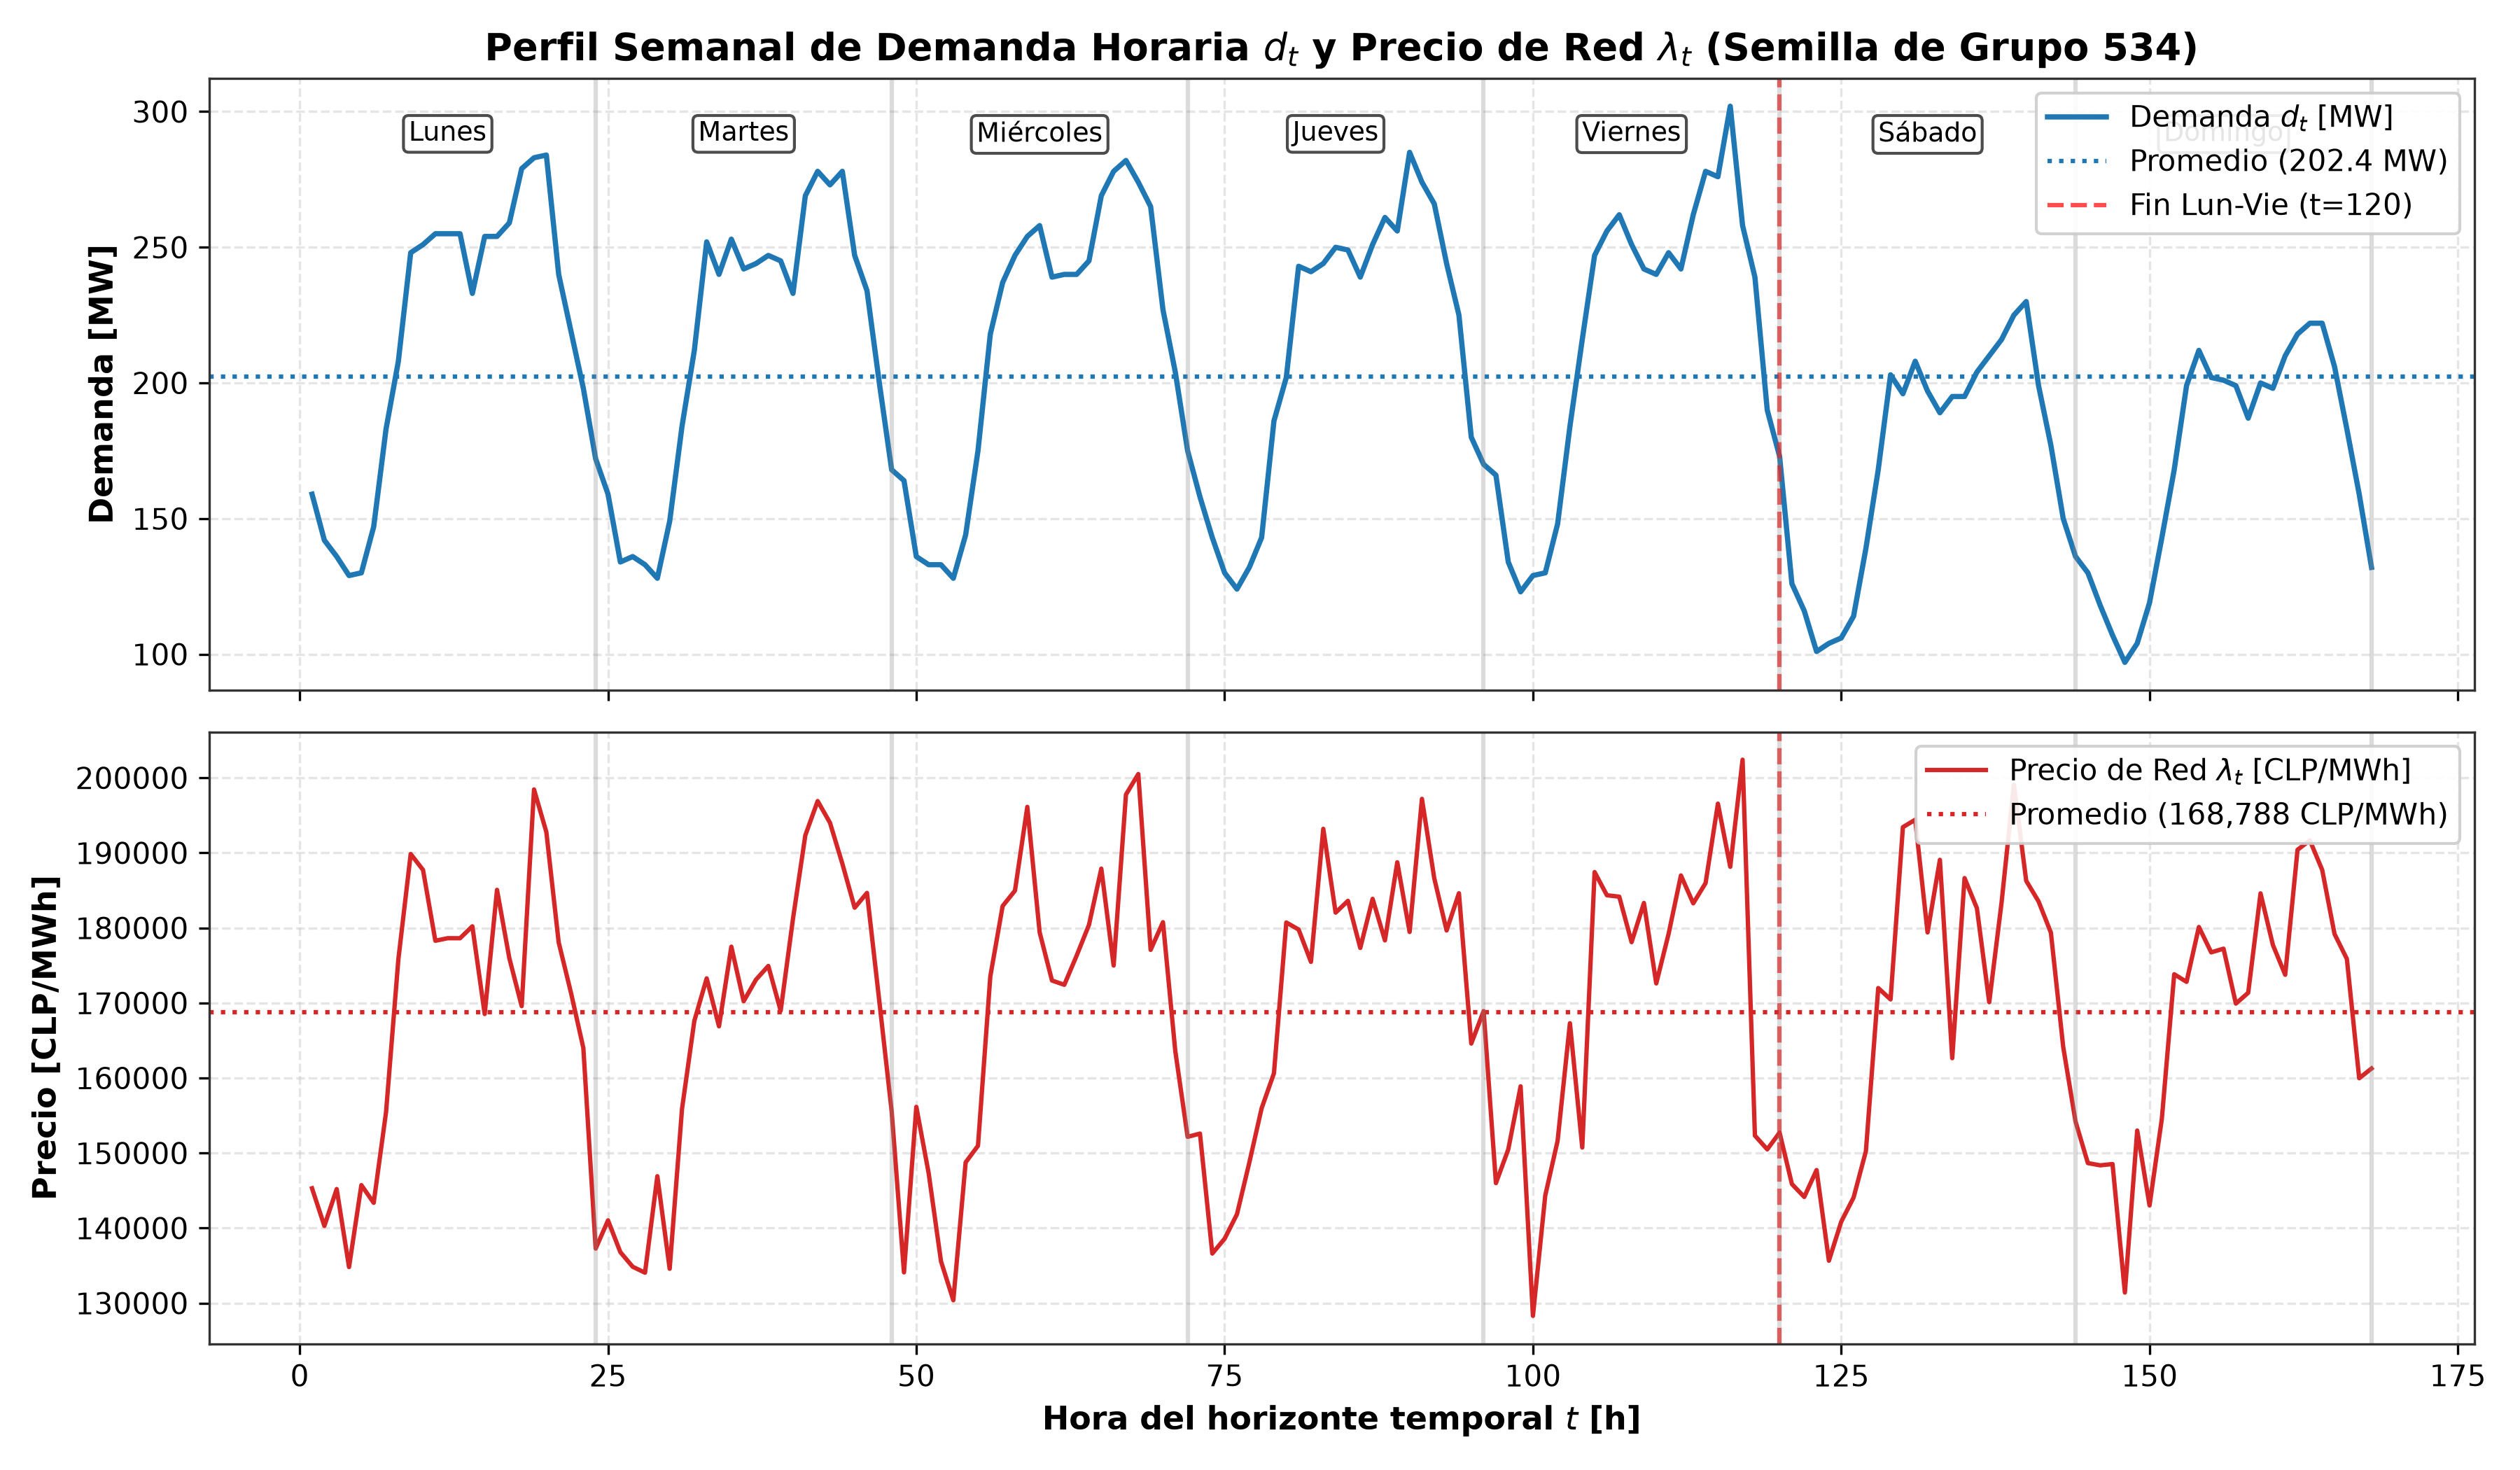
\includegraphics[height=7.5cm,width=0.92\linewidth]{figuras/fig_1a_demanda_precios_sem_534.png}
\caption{Perfiles semanales de demanda horaria $d_t$ y precio de importación de la red $\lambda_t$.}
\label{fig:1a_perfiles}
\end{figure}

\subsection{Pregunta 1.b: Modelamiento del enunciado}
\label{subsec:1b}

\subsubsection*{1. Conjuntos e Índices}
\begin{itemize}
    \item $t \in T = \{1, 2, \ldots, 168\}$: Conjunto de horas del horizonte semanal de planificación.
    \item $g \in G = \{\texttt{Gas\_Base\_1}, \texttt{Gas\_Base\_2}, \texttt{Diesel\_Med\_1}, \texttt{Diesel\_Med\_2}, \texttt{Peaker}\}$: Conjunto de unidades generadoras térmicas.
\end{itemize}

\subsubsection*{2. Parámetros}
\begin{itemize}
    \item $P_g^{max}, P_g^{min}$: Potencia máxima y mínima técnica de la unidad $g$ [MW].
    \item $c_g^{var}$: Costo variable de generación de la unidad $g$ [CLP/MWh].
    \item $c_g^{nl}$: Costo fijo horario de operación en vacío (\textit{no-load}) de la unidad $g$ [CLP/h].
    \item $c_g^{start}$: Costo de arranque de la unidad $g$ [CLP].
    \item $R_g$: Rampa máxima de subida y bajada de la unidad $g$ [MW/h].
    \item $u_g^0, p_g^0$: Estado de encendido inicial (1 o 0) y potencia inicial [MW] de la unidad $g$ en $t=0$.
    \item $\bar{G}_{red}$: Capacidad máxima de importación desde la red externa [MW] ($\bar{G}_{red} = 80$ MW).
    \item $d_t$: Demanda eléctrica para la hora $t$ [MW].
    \item $\lambda_t$: Precio de importación de energía eléctrica desde la red en la hora $t$ [CLP/MWh].
    \item $Res_t$: Reserva mínima requerida en la hora $t$ [MW] ($Res_t = \lfloor 0.10 \cdot d_t \rceil$).
    \item $SU_g, SD_g$: Límite de rampa al arranque y parada de la unidad $g$ [MW], definido como $\max(P_g^{min}, R_g)$.
\end{itemize}

\subsubsection*{3. Variables de Decisión}
\begin{itemize}
    \item $u_{g,t} \in \{0, 1\}$: Variable binaria de compromiso; 1 si la unidad $g$ está encendida en la hora $t$, 0 si está apagada.
    \item $v_{g,t} \ge 0$: Variable continua indicadora de arranque; toma el valor 1 si la unidad $g$ arranca en la hora $t$, 0 e.o.c.
    \item $p_{g,t} \ge 0$: Potencia eléctrica generada por la unidad $g$ en la hora $t$ [MW].
    \item $g_t^{red} \ge 0$: Potencia eléctrica importada desde la red externa en la hora $t$ [MW].
\end{itemize}

\subsubsection*{4. Función Objetivo}
Minimizar el costo total de operación del complejo industrial a lo largo de la semana:
\begin{equation}
    \min Z = \sum_{t \in T} \left( \sum_{g \in G} \left( c_g^{var} \cdot p_{g,t} + c_g^{nl} \cdot u_{g,t} + c_g^{start} \cdot v_{g,t} \right) + \lambda_t \cdot g_t^{red} \right)
    \label{eq:fo_base}
\end{equation}

\subsubsection*{5. Restricciones}
\begin{enumerate}[label=\textbf{R\arabic*.}]
    \item \textbf{Lógica de Arranque de Generadores:}
    \begin{align}
        v_{g,1} &\ge u_{g,1} - u_g^0, \quad \forall g \in G \label{eq:startup_t1} \\
        v_{g,t} &\ge u_{g,t} - u_{g,t-1}, \quad \forall g \in G, \, t \in T \setminus \{1\} \label{eq:startup_t}
    \end{align}
    \textit{Explicación:} Dado que $c_g^{start} > 0$ en la minimización, cuando la unidad pasa de apagado ($u_{g,t-1}=0$) a encendido ($u_{g,t}=1$), el lado derecho es 1, obligando a $v_{g,t}=1$. Si la unidad se mantiene encendida o se apaga, la cota inferior $v_{g,t} \ge 0$ permite óptimamente que $v_{g,t}=0$.
    
    \item \textbf{Límites Técnicos de Capacidad de Generación:}
    \begin{equation}
        P_g^{min} \cdot u_{g,t} \le p_{g,t} \le P_g^{max} \cdot u_{g,t}, \quad \forall g \in G, \, t \in T \label{eq:p_bounds}
    \end{equation}
    \textit{Explicación:} Si la unidad está apagada ($u_{g,t}=0$), se fuerza $p_{g,t}=0$. Si está encendida ($u_{g,t}=1$), la potencia generada debe situarse estrictamente en el rango técnico $[P_g^{min}, P_g^{max}]$.
    
    \item \textbf{Rampas de Subida y Bajada con Ajuste al Arranque/Parada:}
    \begin{align}
        p_{g,t} - p_{g,t-1} &\le R_g \cdot u_{g,t-1} + SU_g \cdot (1 - u_{g,t-1}), \quad \forall g \in G, \, t \in T \label{eq:ramp_up} \\
        p_{g,t-1} - p_{g,t} &\le R_g \cdot u_{g,t} + SD_g \cdot (1 - u_{g,t}), \quad \forall g \in G, \, t \in T \label{eq:ramp_down}
    \end{align}
    (con $p_{g,0} = p_g^0$ y $u_{g,0} = u_g^0$). \\
    \textit{Explicación:} Si la máquina está encendida en periodos consecutivos, la variación de potencia debe ser menor a $R_g$. Al arrancar, la potencia inicial queda acotada por $SU_g = \max(P_g^{min}, R_g)$; combinado con \eqref{eq:p_bounds}, esto permite a las turbinas de gas encender en su mínimo técnico ($P^{min}=40 > R_g=30$) ¿, y a los grupos diésel encender hasta $R_g$. Al detenerse ($u_{g,t}=0$), se exige que en la hora previa la máquina haya bajado a lo más a $SD_g$.
    
    \item \textbf{Balance de Energía (Satisfacción de Demanda):}
    \begin{equation}
        \sum_{g \in G} p_{g,t} + g_t^{red} = d_t, \quad \forall t \in T \label{eq:balance_base}
    \end{equation}
    
    \item \textbf{Reserva Mínima:}
    \begin{equation}
        \sum_{g \in G} \left( P_g^{max} \cdot u_{g,t} - p_{g,t} \right) + \left( \bar{G}_{red} - g_t^{red} \right) \ge Res_t, \quad \forall t \in T \label{eq:reserva_base}
    \end{equation}
    \textit{Explicación:} Exige que la capacidad disponible no utilizada de generadores encendidos más el margen libre de importación de la red externa sumen al menos el 10\% de la demanda horaria. Sustituyendo el balance \eqref{eq:balance_base}, equivale a garantizar que la potencia total en línea satisfaga $\sum P_g^{max} u_{g,t} + \bar{G}_{red} \ge d_t + Res_t$.
    
    \item \textbf{Capacidad de Importación de Red y Naturaleza de Variables:}
    \begin{equation}
        0 \le g_t^{red} \le \bar{G}_{red}, \quad u_{g,t} \in \{0, 1\}, \quad 0 \le v_{g,t} \le 1, \quad p_{g,t} \ge 0, \quad \forall g \in G, \, t \in T \label{eq:naturaleza}
    \end{equation}
\end{enumerate}

\subsection{Pregunta 1.c: Análisis de la Naturaleza del Problema, Solver y Resolución}
\label{subsec:1c}

\subsubsection*{1. Naturaleza Matemática del Problema}
El problema formulado es un \textbf{Programa Lineal Entero Mixto (MILP)} puesto a que ingcluye variables binarias y continuas con relaciones estrictamente lineales.

\subsubsection*{2. Idoneidad del Solver Seleccionado}
Se utilizó el solver de código abierto \textbf{HiGHS} (\texttt{appsi\_highs}), ampliamente usado en investigación operativa. HiGHS resulta óptimo gracias a:
\begin{itemize}
    \item \textbf{Pre-procesamiento Robusto (\textit{Presolve}):} Reduce drásticamente el tamaño del modelo mediante fijación de variables y apriete de cotas.
    \item \textbf{Planos de Corte Especializados:} Incorpora cortes de cliques, residuo mixto entero (MIR) y Gomory, cerrando la brecha de integrabilidad en el nodo raíz.
    \item \textbf{Simplex Dual Multihilo y Heurísticas Primarias:} Acelera la resolución de las relajaciones en cada nodo y descubre rápidamente soluciones enteras factibles de bajo costo.
\end{itemize}

\subsubsection*{3. Resultados de la Resolución Computacional en Pyomo}
En la Tabla \ref{tab:desempeno_solver} se presentan las métricas de resolución y costos desagregados obtenidos para la Semilla 534.

\begin{table}[H]
\centering
\caption{Desempeño del solver HiGHS y costos totales de la solución óptima del Caso Base (Semilla 534).}
\label{tab:desempeno_solver}
\setlength{\tabcolsep}{4pt}
\small
\begin{tabular}{lr}
\toprule
\textbf{Métrica de Optimización} & \textbf{Valor Obtenido (Semilla Oficial 534)} \\
\midrule
Estado de terminación / Gap relativo & Óptimo global probado / 0,00\% \\
Tiempo de cómputo del solver & 0,81 s \\
Variables de decisión / Restricciones & 1.680 (840 binarias, 840 cont.) / 2.184 \\
\midrule
\textbf{Costo Total de Operación [CLP]} & \textbf{\$1.776.019.094,00} \\
-- Costo Variable & \$1.664.741.000,00 (93,73\%) \\
-- Costo Fijo de Operación (\textit{No-Load}) & \$100.060.000,00 (5,63\%) \\
-- Costo de Arranque  & \$7.800.000,00 (0,44\%) \\
-- Costo de Importación de Red Externa & \$3.418.094,00 (0,19\%) \\
\bottomrule
\end{tabular}
\end{table}

\subsection{Pregunta 1.d: Interpretación de Resultados, Orden de Mérito y Reserva}
\label{subsec:1d}

En la Tabla \ref{tab:desglose_unidades_base} y la Figura \ref{fig:1d_despacho_base} se expone el despacho económico detallado para la Semilla Oficial 534.

\begin{table}[H]
\centering
\caption{Despacho y compromiso de unidades en la solución óptima del Caso Base.}
\label{tab:desglose_unidades_base}
\setlength{\tabcolsep}{4pt}
\small
\begin{tabular}{lrrrrrr}
\toprule
\textbf{Unidad Generadora} & \textbf{Costo Var.} & \textbf{Gen. Total} & \textbf{Factor de} & \textbf{Horas en} & \textbf{Número de} & \textbf{Emisiones} \\
& \textbf{[CLP/MWh]} & \textbf{[MWh]} & \textbf{Planta [\%]} & \textbf{Línea [h]} & \textbf{Arranques} & \textbf{[tCO2]} \\
\midrule
\texttt{Gas\_Base\_1} & 45.000 & 19.331,0 & 95,9\% & 168 & 0 & 6.765,8 \\
\texttt{Gas\_Base\_2} & 48.000 & 12.217,0 & 72,7\% & 158 & 2 & 4.642,5 \\
\texttt{Diesel\_Med\_1} & 85.000 & 2.378,0 & 23,6\% & 69 & 5 & 1.545,7 \\
\texttt{Diesel\_Med\_2} & 90.000 & 46,0 & 0,5\% & 2 & 2 & 31,3 \\
\texttt{Peaker} & 120.000 & 18,0 & 0,3\% & 2 & 1 & 13,5 \\
\midrule
\textbf{Importación Red} & Prom. 168.788 & 18,0 & --- & 6 & --- & --- \\
\textbf{Total Sistema} & --- & \textbf{34.008,0} & --- & --- & \textbf{10} & \textbf{12.998,8} \\
\bottomrule
\end{tabular}
\end{table}

\begin{figure}[H]
\centering
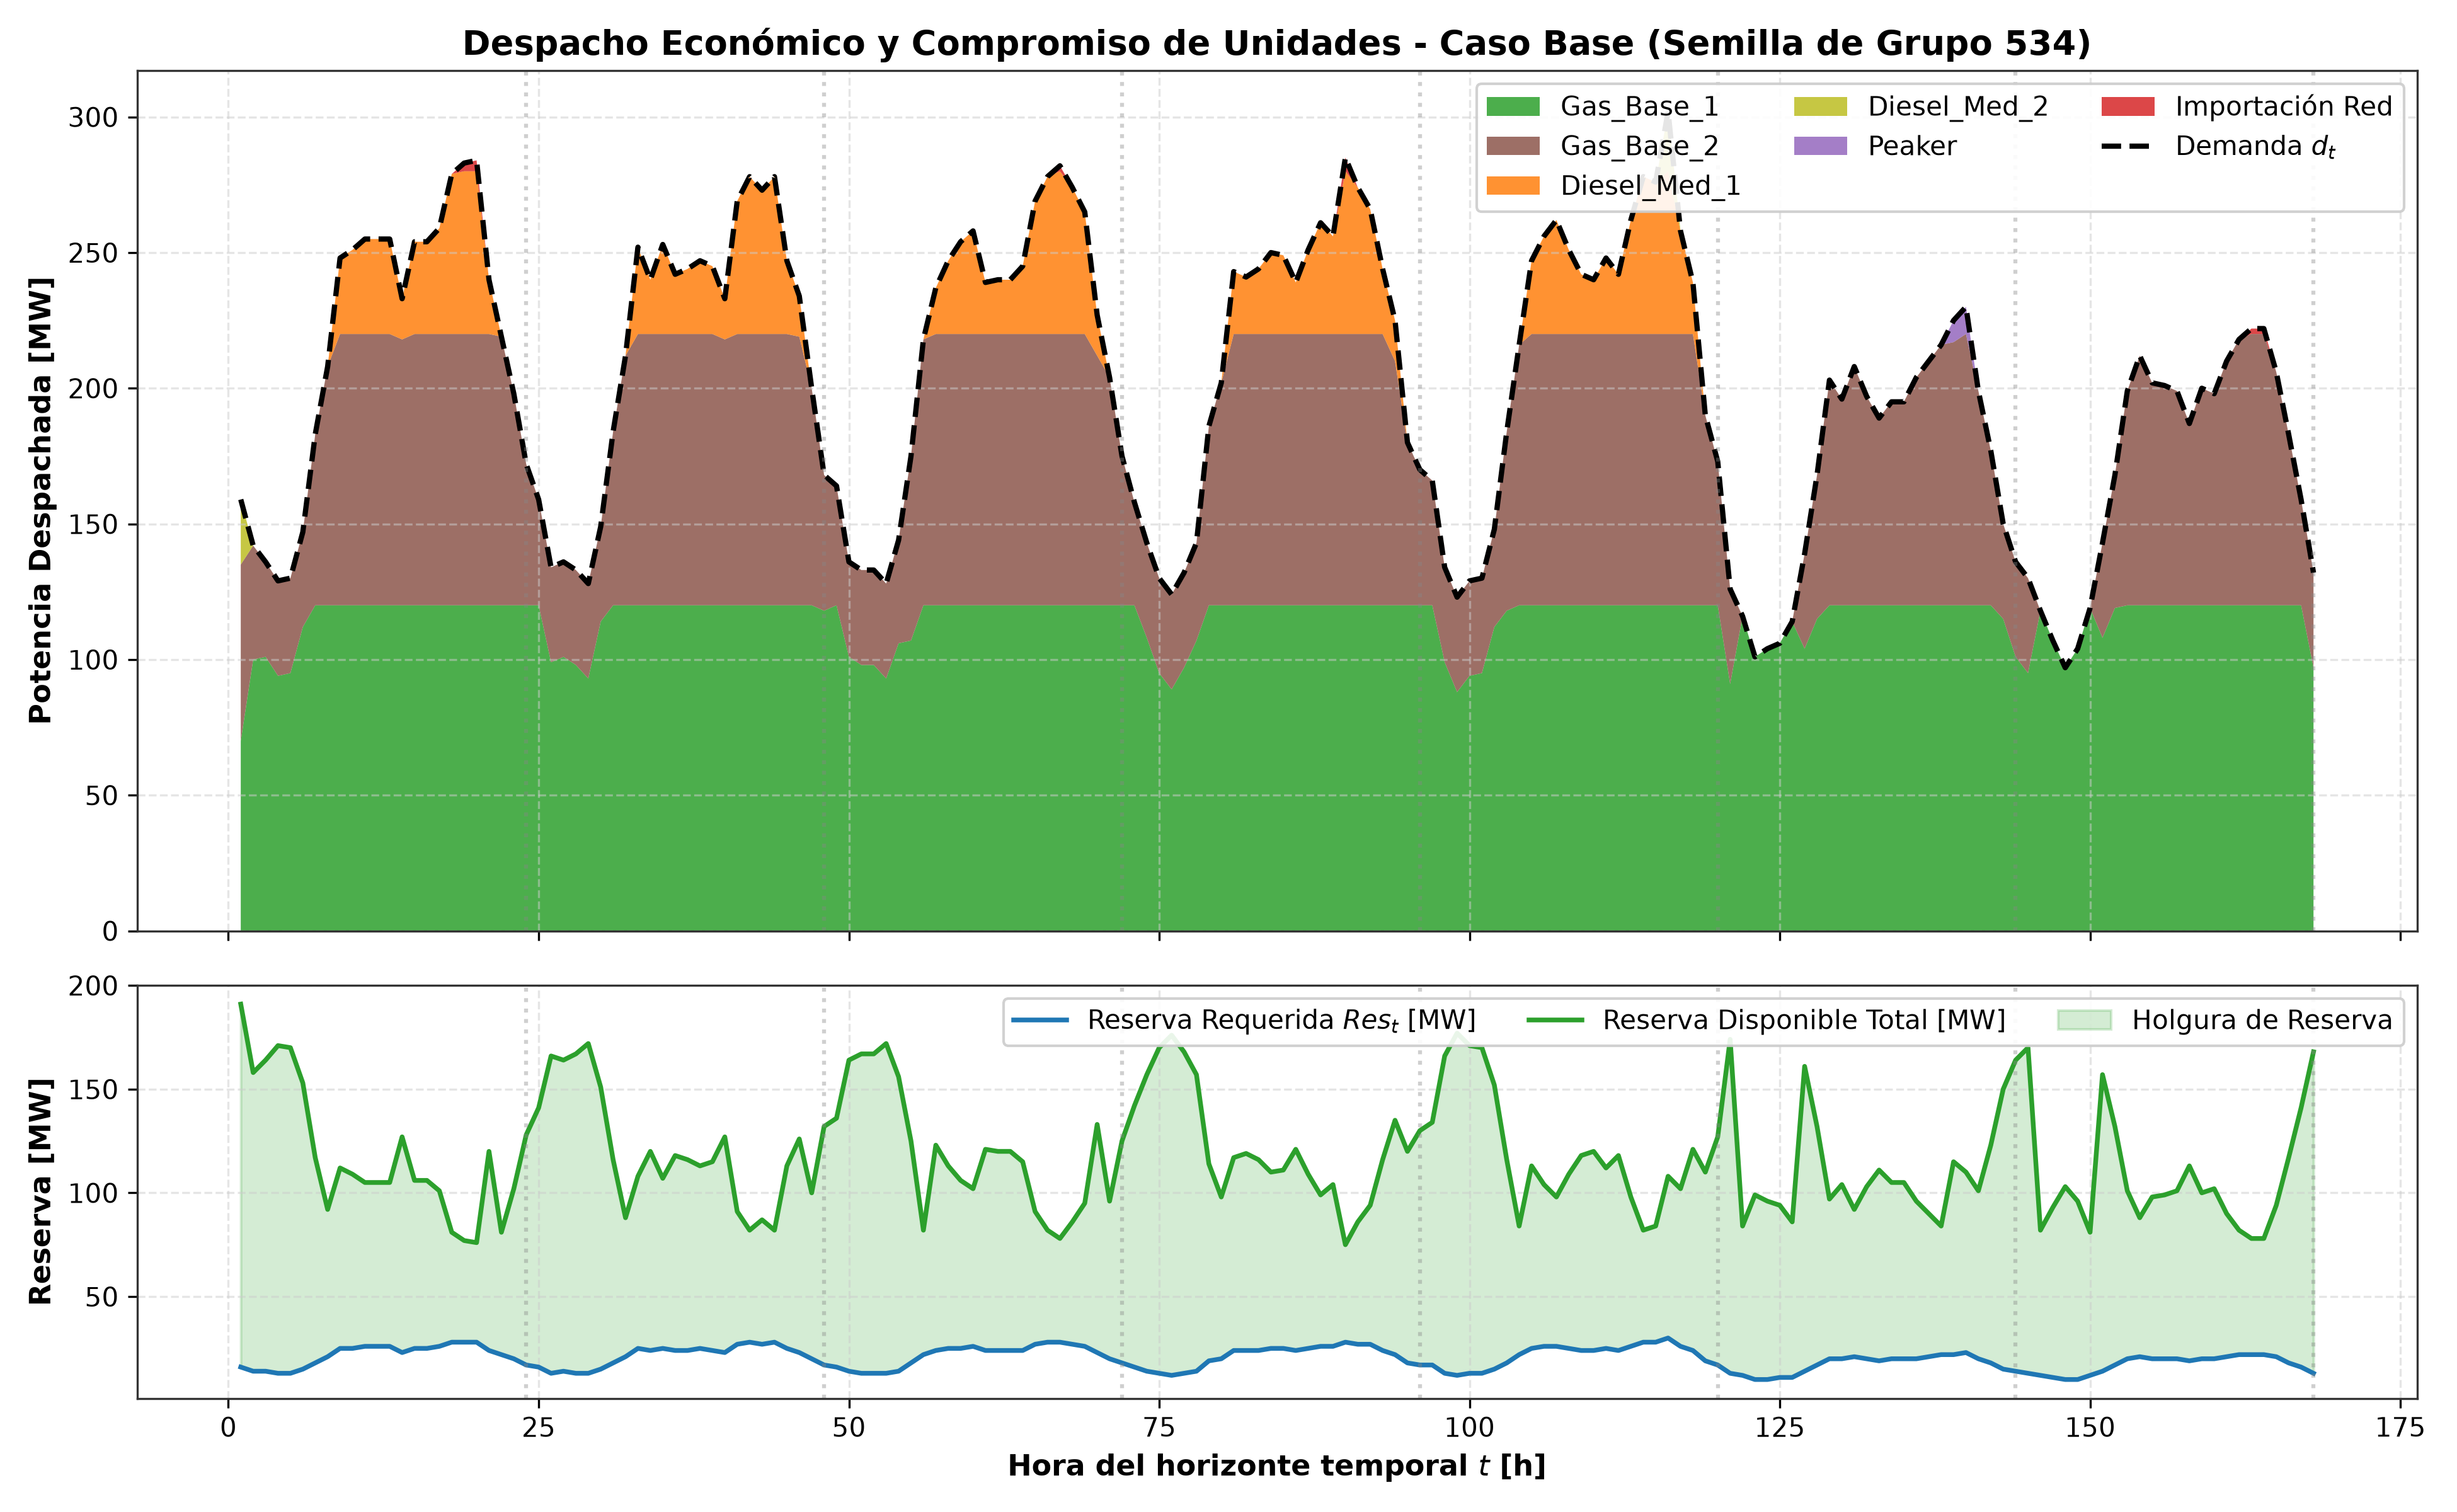
\includegraphics[height=7.5cm,width=0.92\linewidth]{figuras/fig_1d_despacho_base_sem_534.png}
\caption{Despacho económico apilado y reserva operativa horaria en el Caso Base.}
\label{fig:1d_despacho_base}
\end{figure}

El análisis técnico-económico arroja conclusiones fundamentales:
\begin{enumerate}
    \item \textbf{Orden de Mérito Económico:} Se verifica un estricto despacho por mérito de costos variables y de no-load:
    \begin{itemize}
        \item \textit{Unidades de Base:} \texttt{Gas\_Base\_1} opera las 168 horas a plena capacidad (FP 95,9\%), sin arranques. \texttt{Gas\_Base\_2} actúa como segunda base (FP 72,7\%).
        \item \textit{Unidades Intermedias y de Punta:} \texttt{Diesel\_Med\_1} opera en horas laborales de alta carga (5 arranques semanales sincronizados con el inicio diurno). \texttt{Diesel\_Med\_2} y \texttt{Peaker} se reservan exclusivamente para los picos extremos de demanda ($FP \le 0,5\%$).
    \end{itemize}
    \item \textbf{Comportamiento de Arranques:} El modelo evita apagar unidades de gas debido a sus cuantiosos costos de partida (\$2.000.000 y \$1.800.000 CLP), mientras que aprovecha la flexibilidad de las máquinas diésel cuyos costos de arranque (\$600.000 y \$500.000 CLP) son menores.
    \item \textbf{Uso Racionado de la Red Externa:} La importación de red es baja (18,0 MWh en 6 horas). Dado que su costo promedio (\$168.788 CLP/MWh) supera al generador más costoso del complejo (\texttt{Peaker} a \$120.000 CLP/MWh), la red solo se usa ante restricciones de rampa o límites de reserva en picos de demanda.
    \item \textbf{Horas Críticas de Reserva Operativa:} La holgura de reserva ($\text{Reserva Disponible} - Res_t$) se vuelve más exigente en las horas de demanda punta vespertina de días hábiles ($t = 19, 43, 67, 91, 115$), correspondientes a las 18:00--20:00 horas, donde $Res_t$ alcanza 30 MW.
\end{enumerate}

\section{Variaciones}
\label{sec:variaciones}

\subsection{Pregunta 2.a: Incorporación de un Sistema de Almacenamiento}
\label{subsec:2a}

Se integró un sistema de almacenamiento con capacidad de energía $\bar{S} = 200$ MWh, potencia máxima de carga/descarga $\bar{B}^{ch} = \bar{B}^{dis} = 60$ MW, eficiencias $\eta^{ch} = \eta^{dis} = 0.95$ y estado de carga inicial y final mínimo $S_0 = 100$ MWh. Se introducen las variables $p_{ch,t}, p_{dis,t} \in [0, 60]$ y $S_t \in [0, 200]$.

\subsubsection*{Modificaciones Matemáticas al Modelo}
\begin{enumerate}[label=\textbf{R\arabic*.}]
    \setcounter{enumi}{6}
    \item \textbf{Balance de Carga y Condición Final:}
    \begin{align}
        S_t &= S_{t-1} + \eta^{ch} \cdot p_{ch,t} - \frac{p_{dis,t}}{\eta^{dis}}, \quad \forall t \in T \quad (\text{con } S_0 = 100 \text{ MWh}) \label{eq:soc_bal} \\
        S_{168} &\ge S_0 = 100 \text{ MWh} \label{eq:soc_final}
    \end{align}
    \item \textbf{Balance de Energía Modificado para Batería:}
    \begin{equation}
        \sum_{g \in G} p_{g,t} + g_t^{red} + p_{dis,t} = d_t + p_{ch,t}, \quad \forall t \in T \label{eq:bal_bateria}
    \end{equation}
\end{enumerate}

\subsubsection*{Resultados y Análisis Comparativo con el Caso Base}
En la Tabla \ref{tab:comparacion_bateria} y las Figuras \ref{fig:2a_despacho_bateria} y \ref{fig:2a_bateria} se sintetiza el impacto de la batería.

\begin{table}[H]
\centering
\caption{Comparación técnica y económica entre Caso Base y Variación Batería.}
\label{tab:comparacion_bateria}
\setlength{\tabcolsep}{6pt}
\small
\begin{tabular}{lrrr}
\toprule
\textbf{Métrica de Evaluación} & \textbf{Caso Base} & \textbf{Con Batería} & \textbf{Variación Relativa} \\
\midrule
\textbf{Costo Total Semanal [CLP]} & \textbf{\$1.776.019.094} & \textbf{\$1.732.045.839} & \textbf{-2,48\% (-\$43.973.255)} \\
-- Costo Combustible & \$1.664.741.000 & \$1.624.775.839 & -2,40\% \\
-- Costo No-Load & \$100.060.000 & \$99.470.000 & -0,59\% \\
-- Costo Arranque & \$7.800.000 & \$7.800.000 & 0,00\% \\
-- Costo Importación Red & \$3.418.094 & \textbf{\$0} & \textbf{-100,00\%} \\
\midrule
Importación Red Externa [MWh] & 18,0 MWh & \textbf{0,0 MWh} & \textbf{-100,00\%} \\
Energía Cargada / Descargada & --- & 1.225,5 / 1.106,0 MWh & Pérdidas = 119,5 MWh \\
Carga Final ($S_{168}$) [MWh] & --- & 100,0 MWh & Neutro ($\ge 100$) \\
\midrule
\textbf{Arranques Totales de Generadores} & \textbf{10} & \textbf{6} & \textbf{-40,00\% (-4 arranques)} \\
-- \texttt{Diesel\_Med\_2} (Arranques) & 2 & \textbf{0} & \textbf{-100\% (eliminado)} \\
-- \texttt{Peaker} (Arranques) & 1 & \textbf{0} & \textbf{-100\% (eliminado)} \\
-- \texttt{Gas\_Base\_2} (Arranques) & 2 & \textbf{1} & -50\% \\
\bottomrule
\end{tabular}
\end{table}

\begin{figure}[H]
\centering
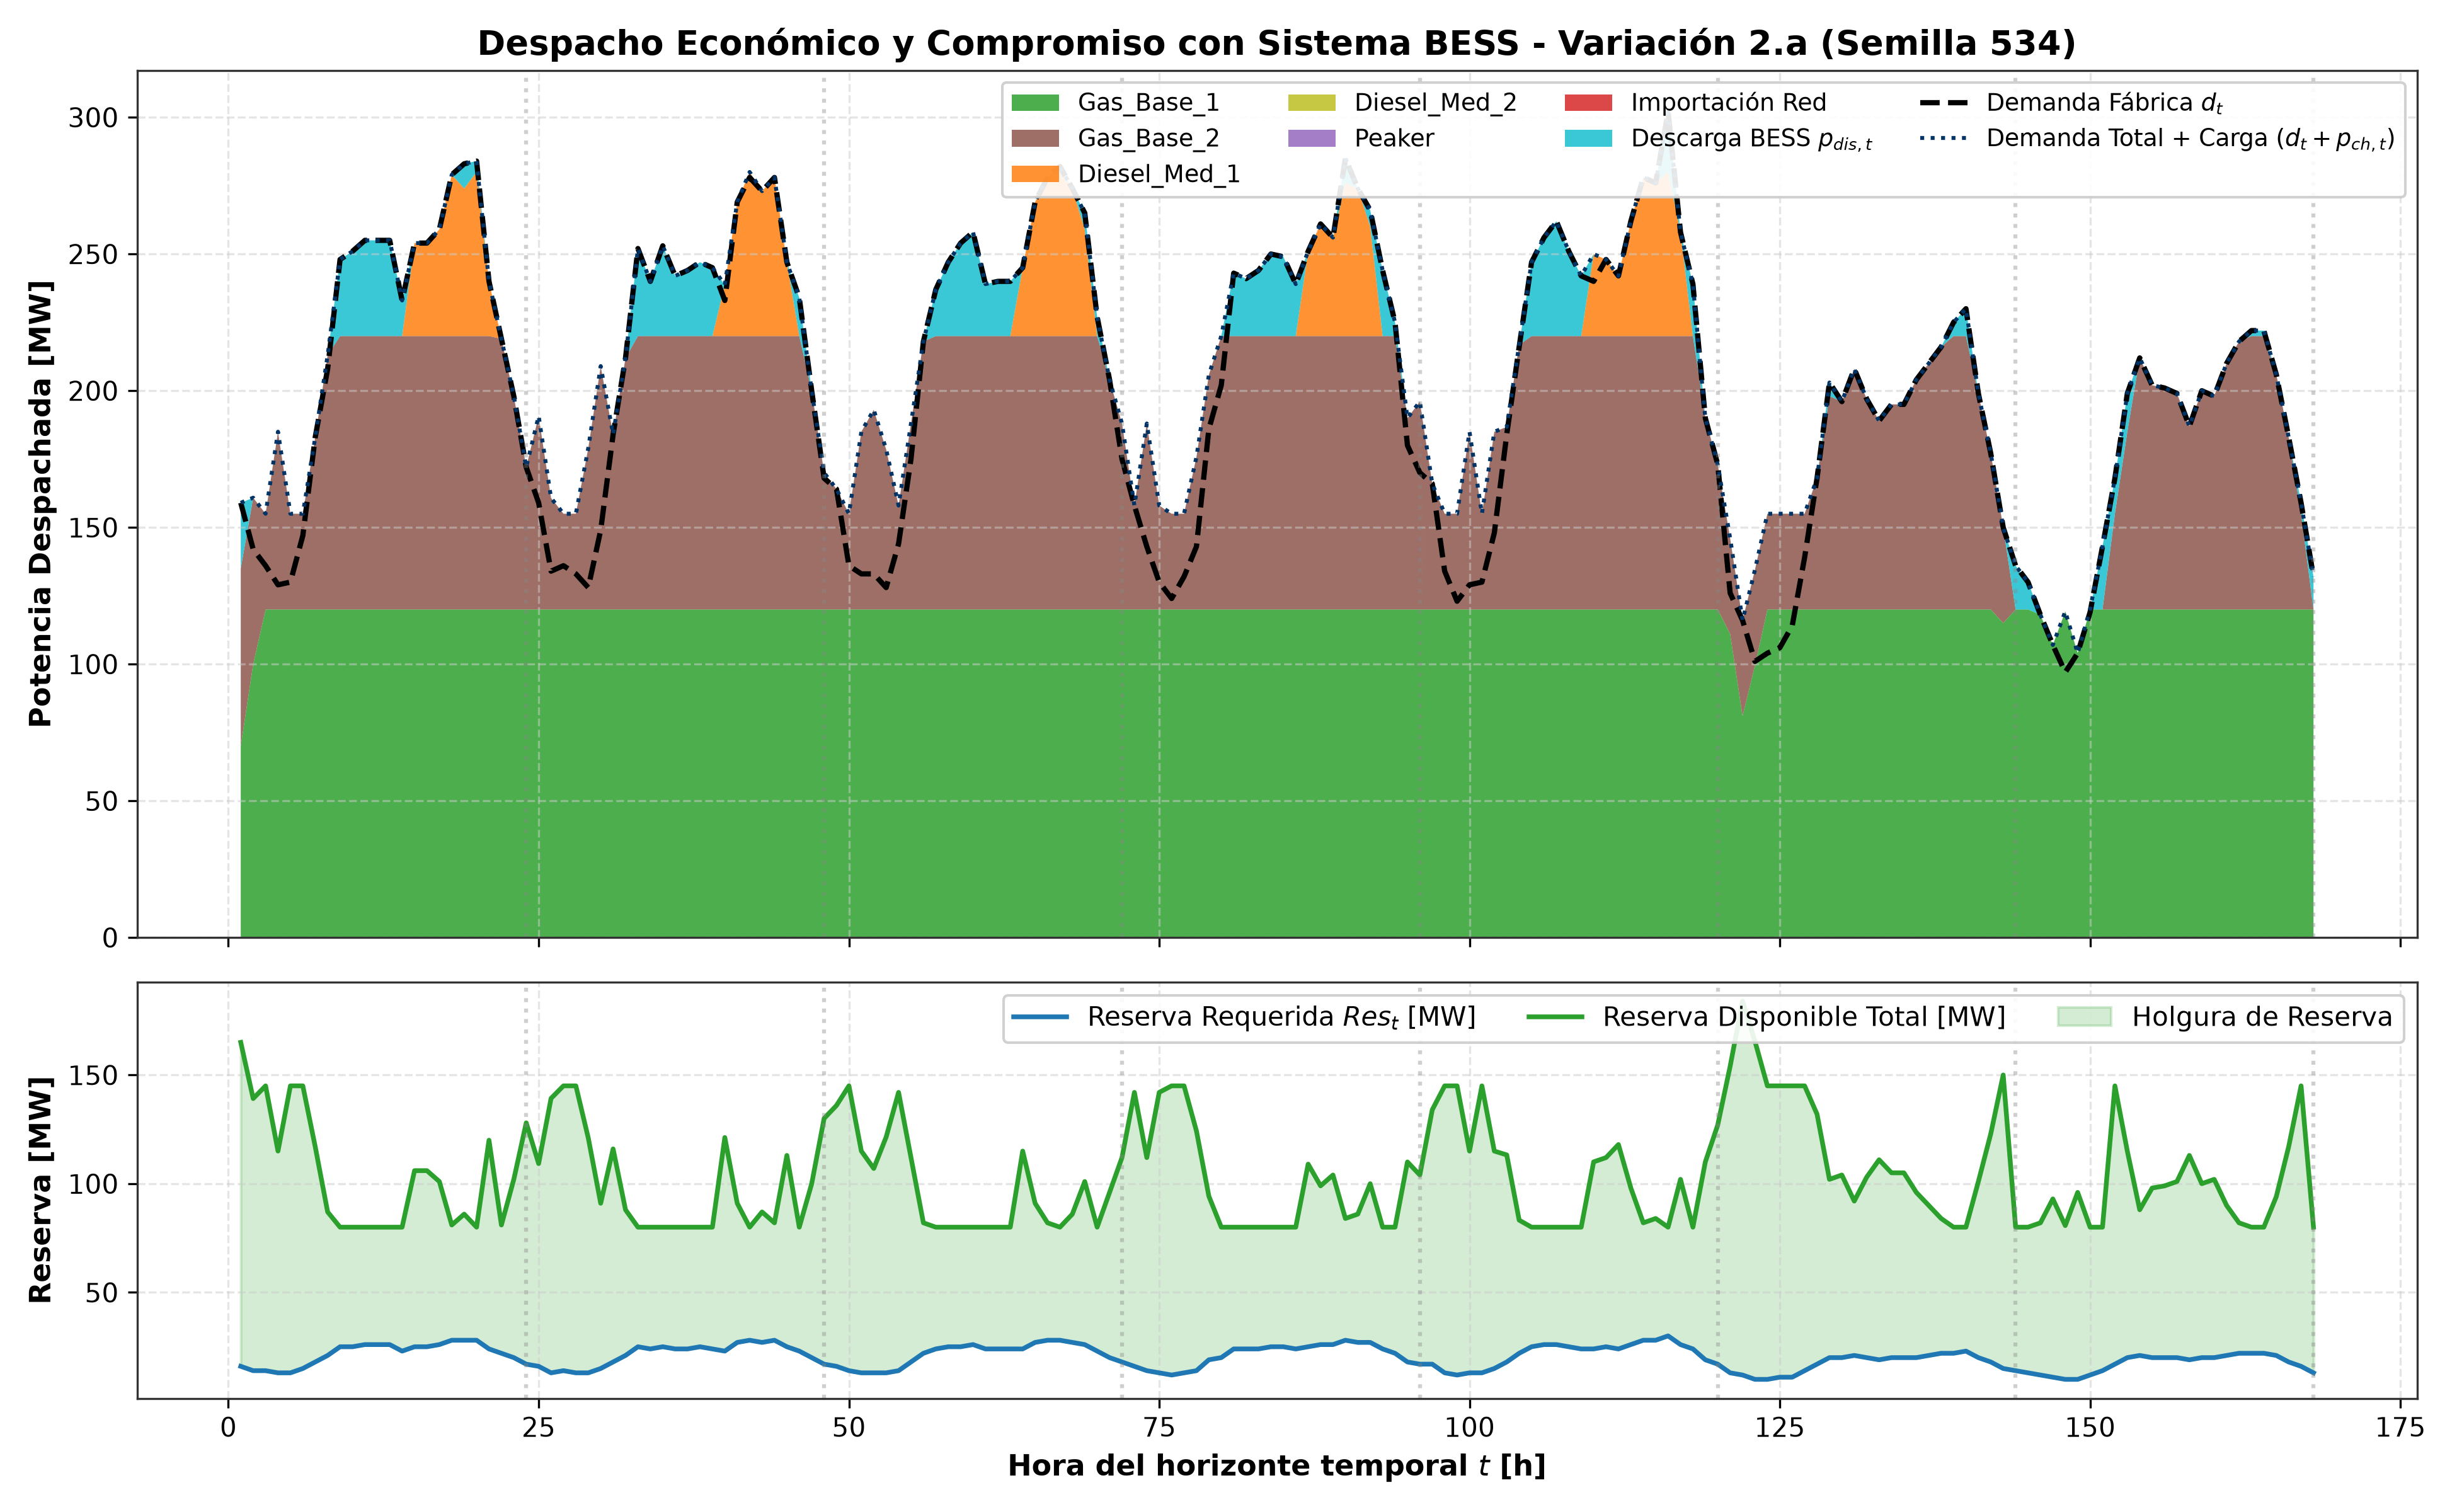
\includegraphics[height=7.0cm,width=0.92\linewidth]{figuras/fig_2a_despacho_bateria_sem_534.png}
\caption{Despacho económico apilado y reserva operativa horaria incorporando el sistema de almacenamiento de energía (Variación 2.a).}
\label{fig:2a_despacho_bateria}
\end{figure}

\begin{figure}[H]
\centering
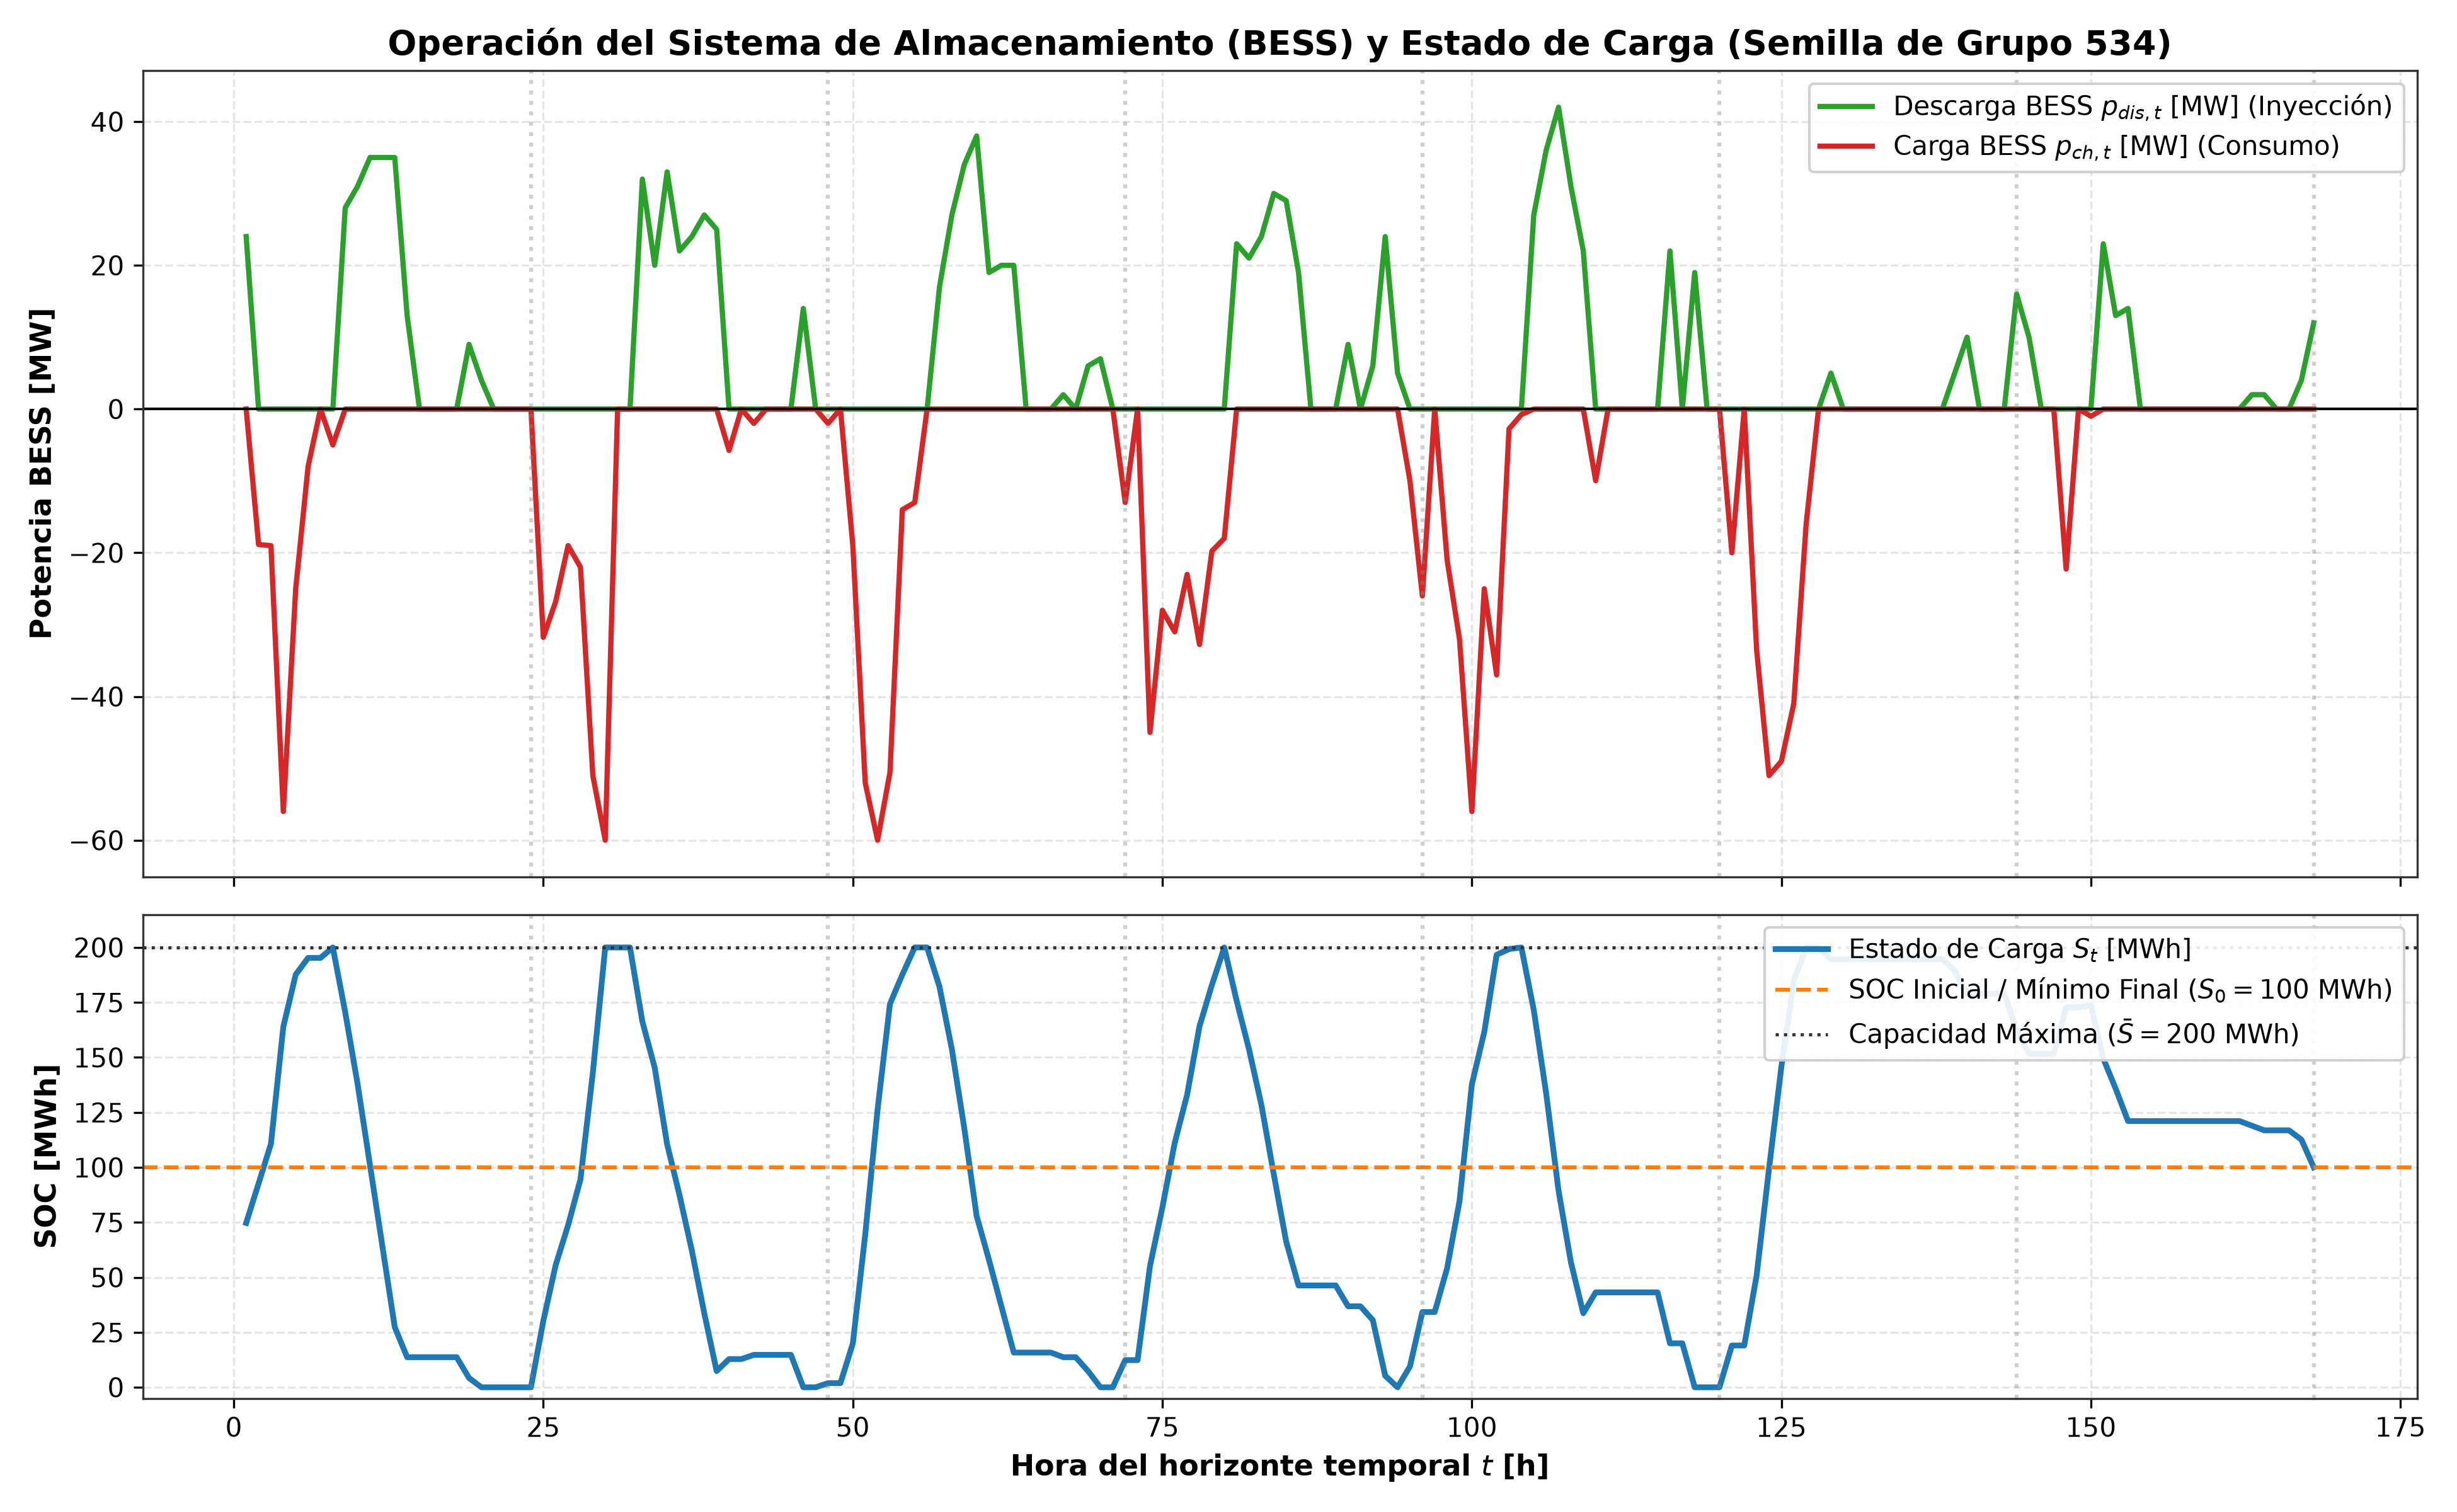
\includegraphics[height=7.0cm,width=0.92\linewidth]{figuras/fig_2a_operacion_bateria_sem_534.png}
\caption{Ciclos de carga, descarga y evolución del estado de carga ($S_t$) de la batería (Semilla 534).}
\label{fig:2a_bateria}
\end{figure}

El análisis operativo revela:
\begin{enumerate}
    \item \textbf{Aplanamiento de Curva de Carga:} La batería almacena energía en horas de la noche-madrugada utilizando capacidad ociosa de las máquinas a gas (\$45.000 CLP/MWh) y la descarga durante los picos de las 18:00--21:00 horas inyectando hasta 60 MW.
    \item \textbf{Eliminación Total de Unidades de Punta y Red Externa:} La batería elimina en un 100\% la importación de red y suprime todos los arranques de \texttt{Diesel\_Med\_2} y \texttt{Peaker}, evitando costosos combustibles y partidas térmicas.
    \item \textbf{Rentabilidad pese a las Pérdidas de Ciclo:} Aunque la eficiencia combinada ($\eta^{ch}\eta^{dis} = 90.25\%$) disipa 119,5 MWh semanales, el diferencial económico entre cargar a \$45.000 y evitar despachos a \$120.000 CLP/MWh genera un ahorro neto de más de \$43,9 millones CLP semanales.
\end{enumerate}

\subsection{Pregunta 2.b: Respuesta de la Demanda (Carga Interrumpible)}
\label{subsec:2b}

Se implementó la variable de recorte $r_t \ge 0$ sujeta a la cota horaria $\bar{\ell}^h = 0.20$ ($r_t \le 0.20 \cdot d_t$) y cuota semanal $\bar{\ell}^s = 0.05$ ($\sum r_t \le 0.05 \sum d_t$), con costo de corte $c^{shed}$ [CLP/MWh].

\subsubsection*{Restricciónes y cambios al modelo}
\begin{itemize}
    \item Balance de energía modificado: $\sum_{g \in G} p_{g,t} + g_t^{red} = d_t - r_t, \quad \forall t \in T$.
    \item Cotas de corte: $r_t \le 0.20 \cdot d_t \quad (\forall t \in T)$ y $\sum_{t=1}^{168} r_t \le 0.05 \cdot \sum_{t=1}^{168} d_t$.
    \item Función objetivo modificada: Se incorpora el término de compensación $+\sum_{t=1}^{168} c^{shed} \cdot r_t$.
\end{itemize}

\subsubsection*{Evaluación Paramétrica y Determinación del Umbral Económico}
En la Tabla \ref{tab:cshed_sweep} y la Figura \ref{fig:variaciones_sensibilidad}(a) se exhiben los resultados del barrido de $c^{shed}$.

\begin{table}[H]
\centering
\caption{Sensibilidad del recorte de demanda y costo total frente a $c^{shed}$ (Cupo = 1.700,4 MWh).}
\label{tab:cshed_sweep}
\setlength{\tabcolsep}{4pt}
\small
\begin{tabular}{rrrrr}
\toprule
$c^{shed}$ \textbf{[CLP/MWh]} & \textbf{Recorte Total [MWh]} & \textbf{Horas con Corte} & \textbf{Costo Operativo [CLP]} & \textbf{Costo Total [CLP]} \\
\midrule
0 & 1.700,4 & 65 & \$1.619.672.142 & \$1.619.672.142 \\
50.000 & 1.700,4 & 66 & \$1.619.672.142 & \$1.704.692.142 \\
80.000 & 1.700,4 & 66 & \$1.619.672.142 & \$1.755.704.142 \\
90.000 & 395,0 & 27 & \$1.735.538.000 & \$1.771.088.000 \\
100.000 & 96,0 & 13 & \$1.762.624.000 & \$1.772.224.000 \\
120.000 & 38,0 & 9 & \$1.769.400.000 & \$1.773.960.000 \\
150.000 & 28,0 & 8 & \$1.770.850.000 & \$1.775.050.000 \\
180.000 & 13,0 & 5 & \$1.773.498.315 & \$1.775.838.315 \\
185.000 & 13,0 & 5 & \$1.773.498.315 & \$1.775.903.315 \\
190.000 & 11,0 & 4 & \$1.773.873.767 & \$1.775.963.767 \\
195.000 & 5,0 & 2 & \$1.775.028.193 & \$1.776.003.193 \\
\textbf{200.000} & \textbf{0,0} & \textbf{0} & \textbf{\$1.776.019.094} & \textbf{\$1.776.019.094} \\
\bottomrule
\end{tabular}
\end{table}

\subsubsection*{Interpretación Microeconómica y Costo Marginal del Sistema}
El corte de carga actúa como un generador virtual. La condición de optimización establece que se corta demanda en la hora $t$ si y sólo si su costo de compensación es inferior al costo marginal del sistema en dicha hora ($c^{shed} < \mu_t$). La curva exhibe tres escalones de saturación:
\begin{enumerate}
    \item Para $c^{shed} \le \$80.000$ CLP/MWh, recortar demanda es más económico que generar con diésel o peaker, saturando el cupo semanal del 5\% (1.700,4 MWh).
    \item Entre \$85.000 y \$120.000 CLP/MWh, el recorte solo sustituye generación diésel marginal y peakers de punta, reduciendo el volumen a 38--395 MWh.
    \item Finalmente, se determina el \textbf{umbral de indiferencia económica exacto}:
    \begin{equation}
        c^{shed*}_{534} = \mathbf{\$200.000 \text{ CLP/MWh}}
    \end{equation}
    Superado este umbral, $c^{shed}$ excede el precio de importación de la red en horas punta vespertinas (cuyo precio máximo alcanza \$202.420 CLP/MWh), haciendo inviable económicamente cualquier recorte ($r_{total} = 0$).
\end{enumerate}

\subsection{Pregunta 2.c: Costo Fijo por Sobrepasar un Umbral Diario de Emisiones}
\label{subsec:2c}

Cada unidad $g$ emite $e_g$ toneladas de $\text{CO}_2$ por MWh generado ($e_g = [0.35, 0.38, 0.65, 0.68, 0.75]$ t$\text{CO}_2$/MWh). Se impone un umbral diario $\bar{E}^{day} = 1.500 \text{ tCO}_2$ durante cada día $d \in \{1, \ldots, 7\}$ , incurriendo en una penalización fija $F$ [CLP/día] en caso de superarlo.

\subsubsection*{Formulación Matemática Big-M}
Se introduce la variable binaria $y_d^{emiss} \in \{0, 1\}$, que indica si el día $d$ supera el umbral:
\begin{enumerate}[label=\textbf{R\arabic*.}]
    \setcounter{enumi}{9}
    \item \textbf{Restricción Disyuntiva Big-M de Emisiones Diarias:}
    \begin{equation}
        \sum_{t \in T_d} \sum_{g \in G} e_g \cdot p_{g,t} - \bar{E}^{day} \le M \cdot y_d^{emiss}, \quad \forall d \in \{1, \ldots, 7\} \label{eq:big_m}
    \end{equation}
    \textit{Determinación del parámetro Big-M:} La emisión física máxima diaria ocurre con las 5 máquinas al 100\% durante 24 horas: $E_{max}^{day} = 24 \times (0.35 \times 120 + 0.38 \times 100 + 0.65 \times 60 + 0.68 \times 50 + 0.75 \times 40) = 4.392 \text{ tCO}_2$. Por ende, la cota superior del exceso es $4.392 - 1.500 = 2.892 \text{ tCO}_2$. Se establece $M = 3.000 \text{ tCO}_2$.
    \item \textbf{Función Objetivo con Penalización Ambiental:}
    \begin{equation}
        \min Z_{emiss} = Z_{base} + \sum_{d=1}^7 F \cdot y_d^{emiss} \label{eq:fo_emiss}
    \end{equation}
\end{enumerate}

\subsubsection*{Evaluación Paramétrica y Tipping Points de Cumplimiento}
En la Tabla \ref{tab:F_sweep} y la Figura \ref{fig:variaciones_sensibilidad}(b) se reporta el barrido paramétrico de $F \in [0, 200.000.000]$ CLP/día.

\begin{table}[H]
\centering
\caption{Sensibilidad de días sobre el umbral de emisiones y costos frente a la penalización $F$.}
\label{tab:F_sweep}
\setlength{\tabcolsep}{4pt}
\small
\begin{tabular}{rrrrr}
\toprule
$F$ \textbf{[CLP/día]} & \textbf{Días Sobre Umbral} & \textbf{Costo Operativo [CLP]} & \textbf{Costo Penalidad [CLP]} & \textbf{Emisiones Totales [tCO2]} \\
\midrule
0 & 5 & \$1.776.019.094 & \$0 & 12.998,8 \\
1.000.000 & 5 & \$1.776.019.094 & \$5.000.000 & 12.998,8 \\
5.000.000 & 5 & \$1.776.019.094 & \$25.000.000 & 12.998,1 \\
10.000.000 & 5 & \$1.776.019.094 & \$50.000.000 & 12.998,8 \\
50.000.000 & 5 & \$1.776.019.094 & \$250.000.000 & 12.998,1 \\
75.000.000 & 5 & \$1.776.019.094 & \$375.000.000 & 12.998,8 \\
\textbf{100.000.000} & \textbf{2} & \textbf{\$2.068.808.322} & \textbf{\$200.000.000} & \textbf{11.513,6} \\
\textbf{120.000.000} & \textbf{0} & \textbf{\$2.276.564.145} & \textbf{\$0} & \textbf{10.467,9} \\
150.000.000 & 0 & \$2.276.442.484 & \$0 & 10.467,9 \\
200.000.000 & 0 & \$2.276.402.498 & \$0 & 10.467,9 \\
\bottomrule
\end{tabular}
\end{table}

\begin{figure}[H]
\centering
\begin{subfigure}[b]{0.48\linewidth}
    \centering
    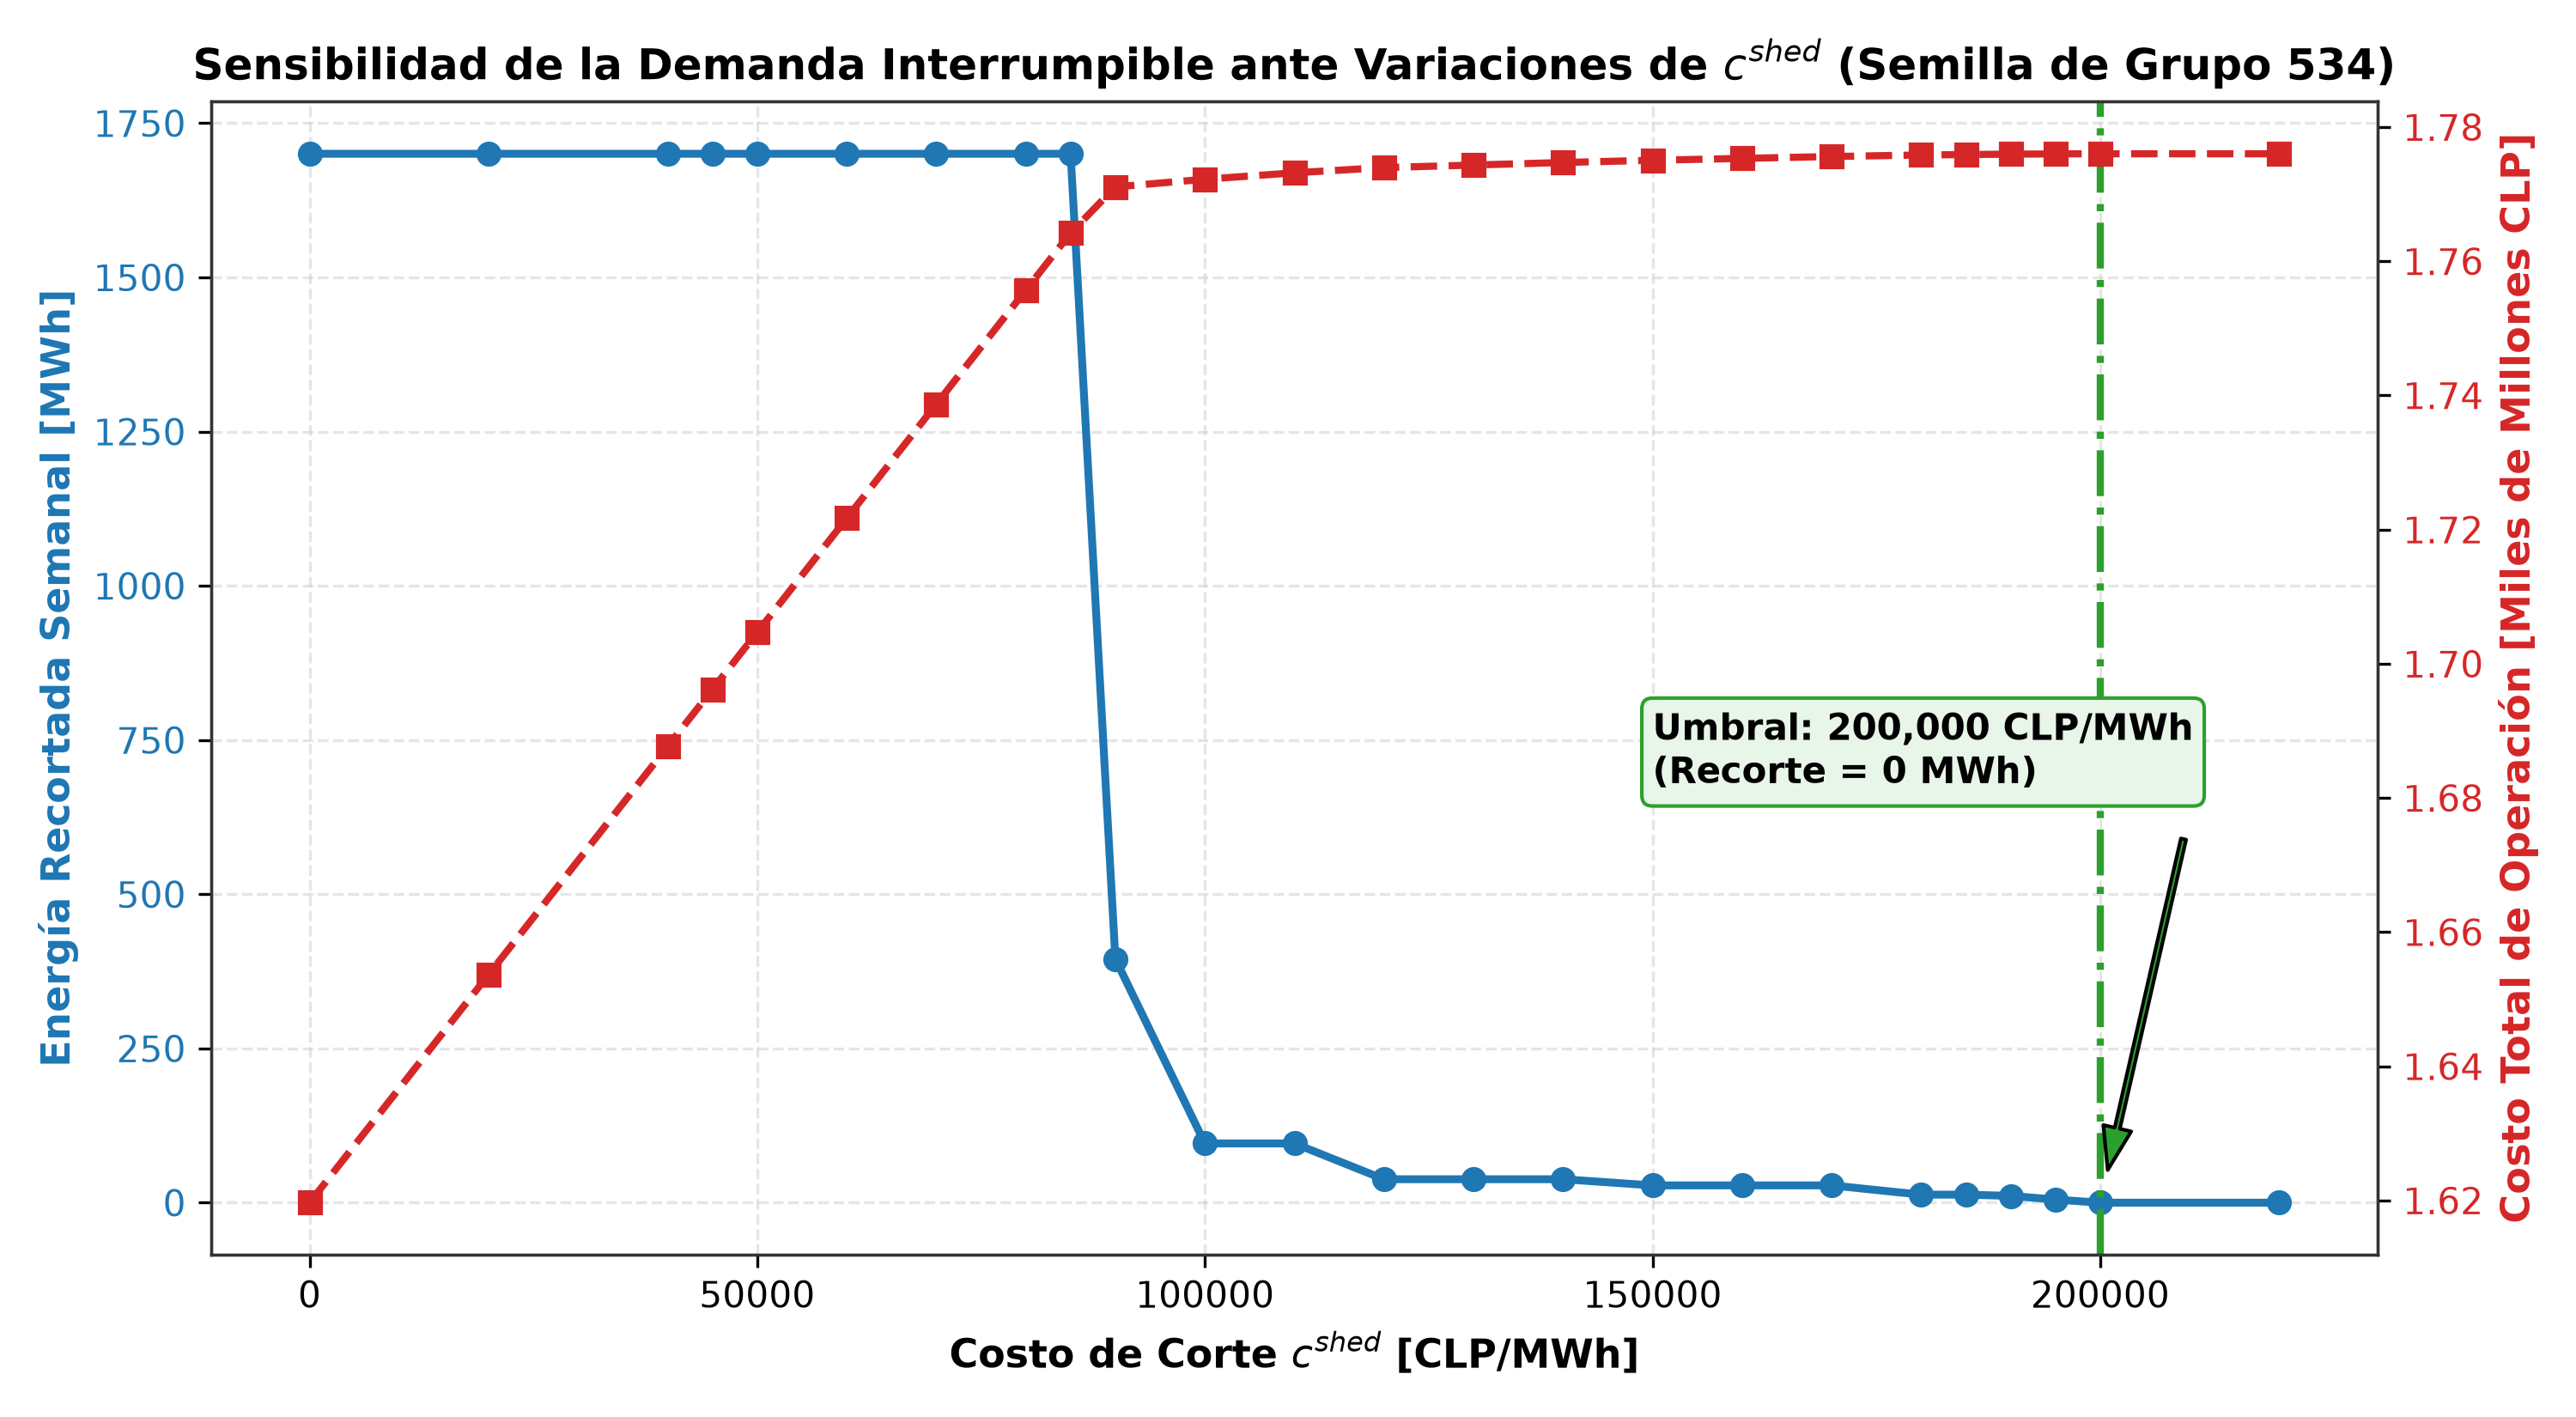
\includegraphics[width=\linewidth]{figuras/fig_2b_demanda_curt_vs_cshed_sem_534.png}
    \caption{Curva de demanda interrumpible vs $c^{shed}$.}
    \label{fig:2b_curt}
\end{subfigure}
\hfill
\begin{subfigure}[b]{0.48\linewidth}
    \centering
    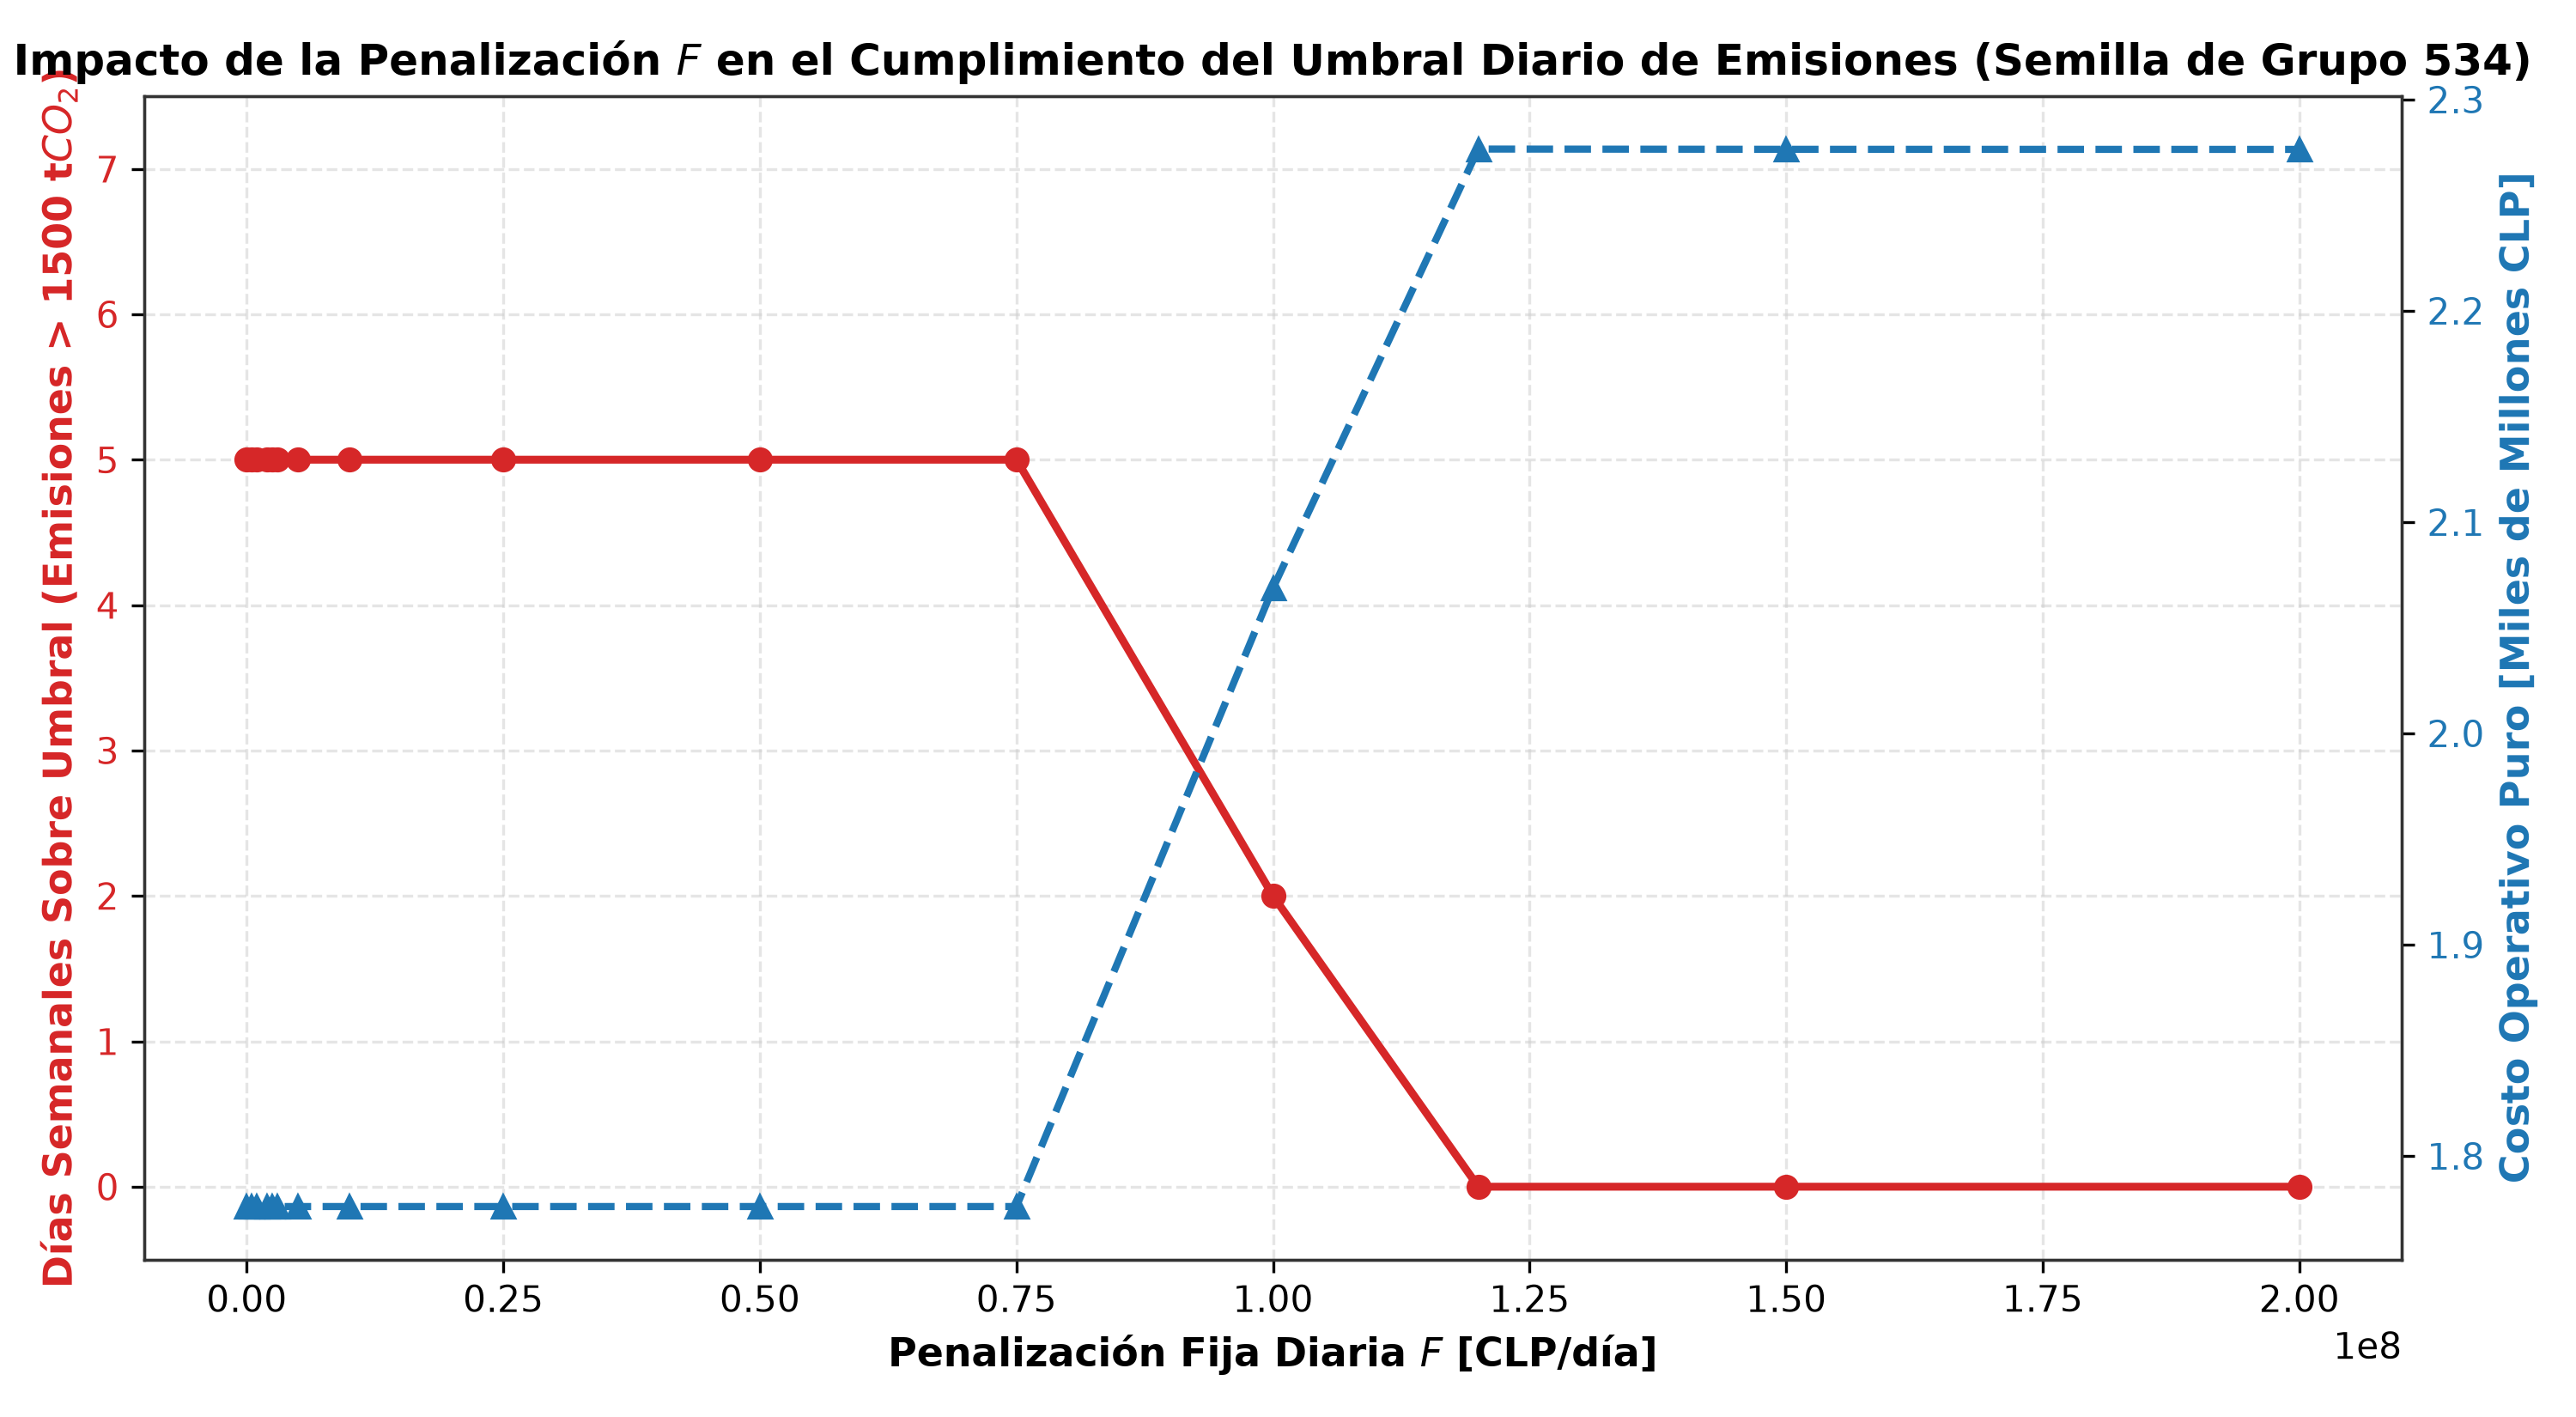
\includegraphics[width=\linewidth]{figuras/fig_2c_emisiones_vs_F_sem_534.png}
    \caption{Días sobre umbral de emisiones vs penalización $F$.}
    \label{fig:2c_F}
\end{subfigure}
\caption{Sensibilidad paramétrica para las variaciones 2.b (Carga Interrumpible) y 2.c (Penalización de Emisiones $F$).}
\label{fig:variaciones_sensibilidad}
\end{figure}

\subsubsection*{Discusión de Implicancias Técnicas y Regulatorias}
El comportamiento del sistema revela conclusiones de alto valor regulatorio:
\begin{enumerate}
    \item \textbf{Cumplimiento Natural en Fines de Semana:} A diferencia de otras instancias con mayor demanda peak, los días sábado y domingo (días 6 y 7) emiten en el caso base $1.483,8$ y $1.487,2\text{ tCO}_2$, situándose por debajo del umbral de 1.500 $\text{tCO}_2$** debido al factor $\gamma_{dia} = 0.8$. Por ello, para cualquier $F \le \$75.000.000$ CLP/día, el número de días infractores es exactamente 5.
    \item \textbf{Tipping Points de Cumplimiento en Días Laborales:} En días hábiles, la demanda diaria supera los $5.100$ MWh, generando sobre $2.000 \text{ tCO}_2$. Bajar a $1.500 \text{ tCO}_2$ exige importar masivamente de la red a su tope de 80 MW/h todo el día ($1.920$ MWh/día). Dado que cada MWh importado cuesta $\approx \$169.000$ CLP mientras que el gas propio cuesta $\approx \$45.000$ CLP, el sobrecosto diario supera los \textbf{\$100 millones CLP por día hábil}. En consecuencia:
    \begin{itemize}
        \item A $F = \$100.000.000$ CLP/día, el sistema comienza a abatir y reduce de 5 a 2 días infractores.
        \item A $F \ge \$120.000.000$ CLP/día, se alcanza el cumplimiento pleno (0 días sobre el umbral), con un costo operativo que pasa de \$1.776 millones a \$2.276 millones CLP semanales.
    \end{itemize}
\end{enumerate}

\section{Conclusiones}
\label{sec:conclusiones}

El desarrollo computacional y analítico de la presente Tarea Computacional 1 ha permitido obtener conclusiones determinantes para la toma de decisiones en micro-redes y despacho eléctrico:
\begin{enumerate}
    \item \textbf{Efectividad del Modelamiento MILP:} El modelo de Unit Commitment formulado capturó con fidelidad matemática las restricciones físicas complejas de rampas dinámicas, costos de partida y márgenes de reserva rodante. La implementación en Pyomo resuelta mediante el solver HiGHS garantizó la optimalidad global estricta en menos de un segundo.
    \item \textbf{Despacho por Orden de Mérito:} La jerarquía de costos variables y costos fijos de no-load gobernó la operación. Las máquinas a gas son el pilar de base con factores de carga superiores al 72\%, mientras que las máquinas diésel proporcionan la agilidad de rampa y seguimiento de carga diurna.
    \item \textbf{Valor del Almacenamiento :} La batería demostró ser una inversión con alto impacto operacional y financiero, logrando ahorros inmediatos de \$43.973.255 CLP semanales (2,48\%) y blindando al complejo industrial frente a la volatilidad de los precios de la red externa mediante la eliminación total de arranques peakers y de importaciones de red.
    \item \textbf{Consistencia Microeconómica de la Demanda Interrumpible:} Se comprobó rigurosamente que el recorte voluntario de demanda cesa exactamente en el costo marginal máximo de importación (\$200.000 CLP/MWh), validando los principios económicos de formación de precios en sistemas eléctricos.
    \item \textbf{Diseño de Mecanismos Ambientales:} Se evidenció que las sanciones fijas diarias por umbral de emisiones conllevan distorsiones severas e incrementos desproporcionados de costos, recomendándose a los tomadores de decisión la adopción de tributos lineales continuos a las emisiones de $\text{CO}_2$.
\end{enumerate}


% =========================================================================
% ANEXOS TÉCNICOS (Opcional - No cuenta dentro de las 10 páginas)
% =========================================================================
\newpage
\appendix
\section{Anexo: Tablas de Datos Horarios y Verificación Numérica}
\label{sec:anexo}

En esta sección se presentan extractos tabulares de verificación de la solución óptima del Caso Base para las primeras 24 horas del horizonte semanal (Semilla 534), ratificando la satisfacción estricta de las restricciones de balance de potencia, rampas y reserva operativa mínima.

\begin{table}[H]
\centering
\caption{Despacho horario detallado de las primeras 24 horas (Día 1).}
\label{tab:anexo_dia1}
\setlength{\tabcolsep}{3.5pt}
\footnotesize
\begin{tabular}{rrrrrrrrrrr}
\toprule
\textbf{Hora $t$} & \textbf{Demanda} & \textbf{Gas 1} & \textbf{Gas 2} & \textbf{Diesel 1} & \textbf{Diesel 2} & \textbf{Peaker} & \textbf{Red} & \textbf{Res. Req.} & \textbf{Res. Disp.} & \textbf{Holgura} \\
& \textbf{[MW]} & \textbf{[MW]} & \textbf{[MW]} & \textbf{[MW]} & \textbf{[MW]} & \textbf{[MW]} & \textbf{[MW]} & \textbf{[MW]} & \textbf{[MW]} & \textbf{[MW]} \\
\midrule
1 & 159 & 70,0 & 65,0 & 0,0 & 24,0 & 0,0 & 0,0 & 16 & 191,0 & 175,0 \\
2 & 142 & 100,0 & 42,0 & 0,0 & 0,0 & 0,0 & 0,0 & 14 & 158,0 & 144,0 \\
3 & 136 & 101,0 & 35,0 & 0,0 & 0,0 & 0,0 & 0,0 & 14 & 164,0 & 150,0 \\
4 & 129 & 94,0 & 35,0 & 0,0 & 0,0 & 0,0 & 0,0 & 13 & 171,0 & 158,0 \\
5 & 130 & 95,0 & 35,0 & 0,0 & 0,0 & 0,0 & 0,0 & 13 & 170,0 & 157,0 \\
6 & 147 & 112,0 & 35,0 & 0,0 & 0,0 & 0,0 & 0,0 & 15 & 153,0 & 138,0 \\
7 & 183 & 120,0 & 63,0 & 0,0 & 0,0 & 0,0 & 0,0 & 18 & 117,0 & 99,0 \\
8 & 208 & 120,0 & 88,0 & 0,0 & 0,0 & 0,0 & 0,0 & 21 & 92,0 & 71,0 \\
9 & 248 & 120,0 & 100,0 & 28,0 & 0,0 & 0,0 & 0,0 & 25 & 112,0 & 87,0 \\
10 & 251 & 120,0 & 100,0 & 31,0 & 0,0 & 0,0 & 0,0 & 25 & 109,0 & 84,0 \\
11 & 255 & 120,0 & 100,0 & 35,0 & 0,0 & 0,0 & 0,0 & 26 & 105,0 & 79,0 \\
12 & 255 & 120,0 & 100,0 & 35,0 & 0,0 & 0,0 & 0,0 & 26 & 105,0 & 79,0 \\
13 & 255 & 120,0 & 100,0 & 35,0 & 0,0 & 0,0 & 0,0 & 26 & 105,0 & 79,0 \\
14 & 233 & 120,0 & 98,0 & 15,0 & 0,0 & 0,0 & 0,0 & 23 & 127,0 & 104,0 \\
15 & 254 & 120,0 & 100,0 & 34,0 & 0,0 & 0,0 & 0,0 & 25 & 106,0 & 81,0 \\
16 & 254 & 120,0 & 100,0 & 34,0 & 0,0 & 0,0 & 0,0 & 25 & 106,0 & 81,0 \\
17 & 259 & 120,0 & 100,0 & 39,0 & 0,0 & 0,0 & 0,0 & 26 & 101,0 & 75,0 \\
18 & 279 & 120,0 & 100,0 & 59,0 & 0,0 & 0,0 & 0,0 & 28 & 81,0 & 53,0 \\
19 & 283 & 120,0 & 100,0 & 60,0 & 0,0 & 0,0 & 3,0 & 28 & 77,0 & 49,0 \\
20 & 284 & 120,0 & 100,0 & 60,0 & 0,0 & 0,0 & 4,0 & 28 & 76,0 & 48,0 \\
21 & 240 & 120,0 & 100,0 & 20,0 & 0,0 & 0,0 & 0,0 & 24 & 120,0 & 96,0 \\
22 & 219 & 120,0 & 99,0 & 0,0 & 0,0 & 0,0 & 0,0 & 22 & 81,0 & 59,0 \\
23 & 198 & 120,0 & 78,0 & 0,0 & 0,0 & 0,0 & 0,0 & 20 & 102,0 & 82,0 \\
24 & 172 & 120,0 & 52,0 & 0,0 & 0,0 & 0,0 & 0,0 & 17 & 128,0 & 111,0 \\
\bottomrule
\end{tabular}
\end{table}

\end{document}
